\documentclass[aspectratio=169, 9pt]{beamer}

% \transdissolve[duration=0.2] % Only works with Adobe Acrobat

% Some important packages
\usepackage{epstopdf}
\hypersetup{colorlinks=false, allcolors=purple}
\usepackage{booktabs}
\linespread{1.3}
\usepackage{tabularx,multirow}
\usepackage{makecell} % For makecell within tables
\usepackage{geometry}
\usepackage{fancybox}
\usepackage{algorithm2e}
\usepackage{amsmath, amssymb}
% Mathematical functions
% DELETED!
\renewcommand{\Pr}[1]{{\mathbb{P}\left(#1\right) }}
% DELETED!
% DELETED!
% DELETED!
% DELETED!
% DELETED!

% DELETED!
\newcommand{\sufstats}[1]{s\left(#1\right)}
\renewcommand{\exp}[1]{\mbox{exp}\left\{#1\right\}}
\renewcommand{\log}[1]{\mbox{log}\left\{#1\right\}}
\newcommand{\transpose}[1]{{#1}^\mathbf{t}}
\renewcommand{\t}[1]{\transpose{#1}}

\newcommand{\s}[1]{\sufstats{#1}}
\newcommand{\SUFF}{\mathcal{S}}
\newcommand{\Suff}{\mathbf{S}}
\newcommand{\suff}{\mathbf{s}}

\renewcommand{\beta}{\theta}
\newcommand{\weight}{\mathbf{w}}
\newcommand{\Weight}{\mathbf{W}}

% Objects
% DELETED!
% DELETED!
\newcommand{\Graph}{\mathbf{G}}
\newcommand{\graph}{\mathbf{g}}
\newcommand{\GRAPH}{\mathcal{G}}
\newcommand{\Adjmat}{Y}
\newcommand{\adjmat}{y}
\newcommand{\ADJMAT}{\mathcal{Y}}

\newcommand{\INDEPVAR}{\mathcal{X}}
\newcommand{\Indepvar}{X}
\newcommand{\indepvar}{x}

\newcommand{\normconst}{\kappa\left(\params, \Indepvar\right)}

\graphicspath{{./figures/}{.}{./terms/}}


%% NEED THIS FOR CANCY TEX
\usepackage{pstricks}

% Colors
\definecolor{USCCardinal}{HTML}{990000} % 153 0 0 in RGB
\definecolor{USCGold}{HTML}{FFCC00}
\definecolor{USCGray}{HTML}{CCCCCC}

% \bibliography{bibliography.bib}

\def\ergmito{ERGM\textit{ito}}
\def\ergmitos{\ergmito{}\textit{s}}
% Mathematical functions
\newcommand{\isone}[1]{{\boldsymbol{1}\left( #1 \right)}}
\renewcommand{\Pr}[1]{{\mathbb{P}\left(#1\right) }}
\newcommand{\f}[1]{{f\left(#1\right) }}
\newcommand{\Prcond}[2]{{\mathbb{P}\left(#1\vphantom{#2}\;\right|\left.\vphantom{#1}#2\right)}}
\newcommand{\fcond}[2]{{f\left(#1|#2\right) }}
\newcommand{\Expected}[1]{{\mathbb{E}\left\{#1\right\}}}
\newcommand{\ExpectedCond}[2]{{\mathbb{E}\left\{#1\vphantom{#2}\right|\left.\vphantom{#1}#2\right\}}}
\renewcommand{\exp}[1]{\mbox{exp}\left\{#1\right\}}

\newcommand{\Likelihood}[2]{\text{L}\left(#1 \left|\vphantom{#1}#2\right.\right)}

\newcommand{\loglik}[1]{l\left(#1\right)}


% Mathematical Annotation -------------------------------
% Modify this so that it matches the P01 convention overall

% Tree
\newcommand{\phylo}{\Lambda{}} % The actual tree
\newcommand{\aphylo}{D{}}      % The annotated phylogenetic tree
\newcommand{\aphyloObs}{\tilde \aphylo{}} % The observed annotated phylogenetic tree
\newcommand{\parent}[1]{\mathbf{p}\left(#1\right)}
\newcommand{\offspring}[1]{\mathbf{O}\left(#1\right)}
\newcommand{\nodes}{\mathcal{N}{}}
\newcommand{\edges}{\mathcal{E}{}}

\newcommand{\class}[1]{C_{#1}{}}

% Annotations
\newcommand{\Ann}{\mathbf{X}{}} % Matrix of "real" annotations
\newcommand{\ann}[1]{x_{#1}{}} % single element of "real" annotations
\newcommand{\constraints}{\mathcal{C}{}} % Taxon constraints

% Obs Annotations
\newcommand{\AnnObs}{\mathbf{Z}{}}%{Z{}} \mathbf{X}^{obs}{}
\newcommand{\annObs}[1]{z_{#1}{}}%{z{}}  x_{#1}^{obs

% Pred. Annotations
\newcommand{\AnnPred}{\hat X{}}
\newcommand{\annPred}[1]{\hat x_{#1}}

% Leaf nodes
\newcommand{\Leaf}{L{}}

% Shortest path
\newcommand{\Geodesic}{\text{T}{}}
\newcommand{\geodesic}{\tau{}}

\newcommand{\Params}{\Omega{}}
\newcommand{\params}{\omega{}}

% Parameters
\newcommand{\gain}{\mu_{01}{}}
\newcommand{\loss}{\mu_{10}{}}
\newcommand{\misszero}{\psi_{01}{}}
\newcommand{\missone}{\psi_{10}{}}
\newcommand{\proot}{\pi}


\usepackage[style=authoryear-comp]{biblatex}
\addbibresource{bibliography-aphylo.bib}
\addbibresource{bibliography-ergmito.bib}
\addbibresource{bibliography-extra.bib}
\addbibresource{bibliography.bib}
% \renewcommand{\bibsection}{\subsubsection*{\bibname } }


% Styles
\usepackage{xcolor}
\usepackage{colortbl}
\definecolor{suffstat}{RGB}{10,159,0}
\definecolor{normconst}{RGB}{87,38,231}
\setbeamercolor{conclusions}{bg=usclightgray!60!white, fg=uscdarkgray}

% Noice!
\usetheme{usckeck}

\title[Stat. Comp. for Complex Systems]{Essays on Bioinformatics and
Social Network Analysis
\linebreak{\small Statistical and Computational Methods for
Complex Systems}}
\author[GGVY]{George G Vega Yon}
\institute[USC-PREVMED]{University of Southern California, Department of Preventive Medicine}
\date{June 22, 2020}

% Some definitions
\def\cursection{\frame{\frametitle{Contents}\tableofcontents[current]}}
\newcommand{\ergmpkg}[0]{\texttt{ergm}}
\newcommand{\ergmitopkg}[0]{\texttt{ergmito}}
\newcommand{\aphylopkg}[0]{\texttt{aphylo}}
\graphicspath{{.}{fig/}}


% ------------------------------------------------------------------------------
% ------------------------------------------------------------------------------
% --------------------------- END OF PREAMBLE ----------------------------------
% ------------------------------------------------------------------------------
% ------------------------------------------------------------------------------
\setbeamertemplate{note page}[plain]
%\setbeameroption{show notes}
\usepackage{pgfpages}
% \setbeameroption{show notes on second screen}

\newcommand{\hlc}[2]{{\only<#1>{\cellcolor{gray!50}#2}}}
\newcommand{\nhlc}[2]{{\only<#1>{#2}}}
\newcommand{\hlcAlt}[2]{\alt<#1>{\cellcolor{gray!50}#2}{#2}}

\begin{document}

% ------------------------------------------------------------------------------
\begin{frame}%[noframenumbering]
\maketitle
\end{frame}

% ------------------------------------------------------------------------------
\begin{frame}
\frametitle{What motivates my research}

\begin{center}
\large
\textcolor{usccardinal}{\bf Statistical and computational methods for\\ %
bioinformatics and social network analysis}
\end{center}

\begin{itemize}[<+->]
\item We live in a non-{\it IID} world.
\item In some times, the cannot understand a process unless we look at it as a whole.
\item There's a reason why we usually assume {\it IID}.
\item {\it Modern} (as of today) computational tools help us coping with that.
\end{itemize}
\end{frame}


\frame{\frametitle{Contents}\tableofcontents}

% ------------------------------------------------------------------------------
\section{Paper 1: On the prediction of gene functions using phylogenetic trees}

\begin{frame}[t]
\usebeamertemplate{section intro}{}{}
\textcolor{uscgold}{
\Large {\bf On the prediction of gene functions using phylogenetic trees} \vskip0.25em
\large \textit{Joint with}: Paul D Thomas, Paul Marjoram, Huaiyu Mi, Duncan Thomas, and John Morrison
}
\end{frame}

% ------------------------------------------------------------------------------
\begin{frame}
\frametitle{Genes}

Encode the synthesis of genetic products that ultimately are related to a
particular aspect of life, for example

\def\tmpwidth{.9\linewidth}

\begin{table}
\begin{tabular}{*{3}{m{.31\linewidth}<{\centering}}}
\onslide<2->\bf Molecular function & %
\onslide<3->\bf Cellular component & %
\onslide<4->\bf Biological process \\
\onslide<2->\href{http://amigo.geneontology.org/amigo/term/GO:0005215}{Active transport GO:0005215}& %
\onslide<3->\href{http://amigo.geneontology.org/amigo/term/GO:0004016}{Mitochondria GO:0004016} & %
\onslide<4->\href{http://amigo.geneontology.org/amigo/term/GO:0060047}{Heart contraction GO:0060047} \\
\onslide<2->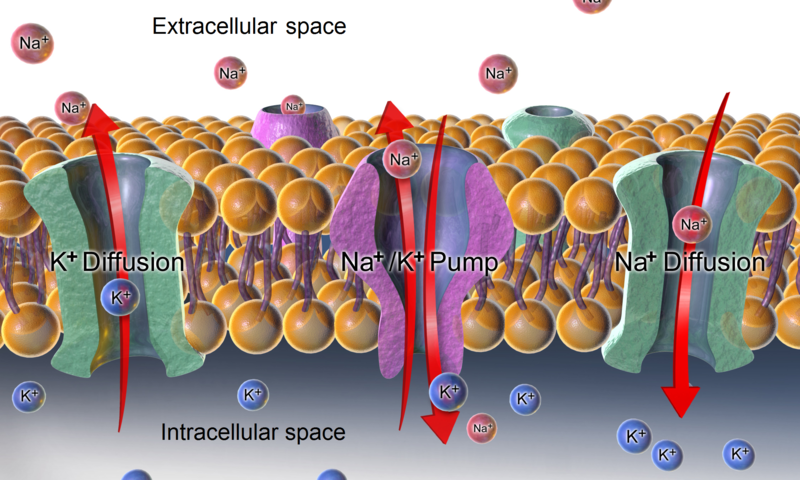
\includegraphics[width=\tmpwidth]{Sodium-potassium_pump_and_diffusion.png} & %
\onslide<3->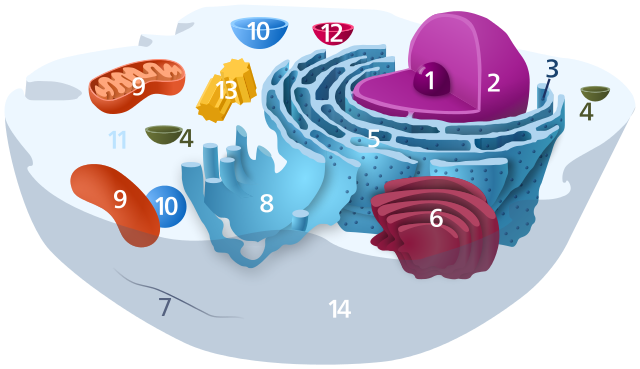
\includegraphics[width=\tmpwidth]{640px-Animal_Cell-svg.png} & % 
\onslide<4->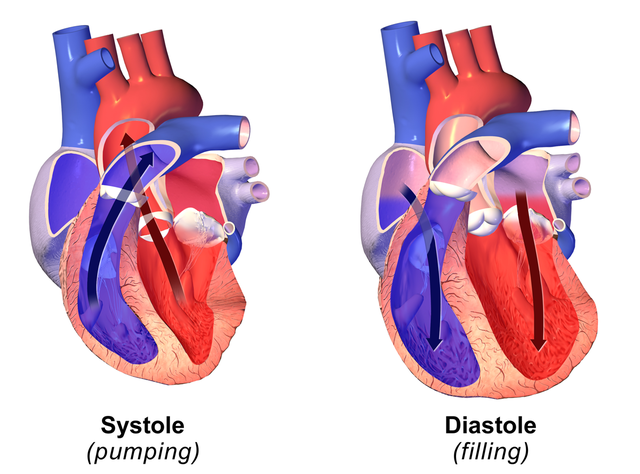
\includegraphics[width=\tmpwidth]{Systolevs_Diastole.png}
\end{tabular}
\end{table}

\end{frame}

\note[enumerate]{
\item Understanding genes means understanding biology
\item Far more than simply pursuing knowledge, this means that we can actually
use this information towards 
}


% ------------------------------------------------------------------------------
\begin{frame}[label=geneontology]
\frametitle{The Gene Ontology Project}

\begin{figure}

\includegraphics[width=.5\linewidth]{go-logo.png}
\end{figure}

\begin{itemize}[<+->]
% \item Three domains: Cellular component, molecular function, biological process.
\item The GO project has $\sim$ 44,700 validated terms  \hyperlink{aphylo-goexample}{\beamergotobutton{more}}, $\sim$ 7.3M annotations on $\sim$ 4,500 species.
\item About $\sim$ 500,000 are on human genes.
\item Roughly half of human genes ($\sim$ 10,000 / 20,000) have some
form of annotation.
\item We know something of less than 10\% of known genes (near 1.7M).
\item An important effort of the GO has to do with phylogenetics...
\end{itemize}

\vfill
\hfill \textbf{source}: Statistics from \url{pantherdb.org} and \url{geneontology.org}

\end{frame}

\note[itemize]{
\item The Gene Ontology Project, which is an international scientific effort to develop
a knowledge base of biology from molecular level up to organism-level systems.
\begin{quote}
[\dots] develop an up-to-date, comprehensive, computational model of biological systems, from the molecular level to larger pathways, cellular and organism-level systems.
\item It has a large collection of genetic annotations from various types of evidence
including: experimentally, human curated information, and machine inferred.
\end{quote}

\item A long way since 1999 (20 years), there's still a lot to learn
\item This information has been crucial for bio-medical research (e.g. translating
GWAS to treatment.)
}



% ------------------------------------------------------------------------------
\begin{frame}

\begin{figure}
\centering
{\footnotesize
\def\svgwidth{.7\linewidth}
\input{fig/Phylogenetic_tree-wiki.pdf_tex}
}
\caption{A phylogenetic tree of living things, based on RNA data and proposed by Carl Woese, showing the separation of bacteria, archaea, and eukaryotes (\href{https://en.wikipedia.org/wiki/File:Phylogenetic_tree.svg}{wiki})}
\end{figure}
\end{frame}

\note[enumerate]{
\item Phylogenetic trees show evolutionary relationships between species
\item Traditionally, we think about these based on say physical features, 
nowadays we build trees based on genetic distances between species.
}



\note[enumerate]{
\item Here we have an example of a (simulated) phylogenetic tree.
\item We will see this a couple of times during the presentation
\item This figure summarizes the information that I will be using
to infer gene functions:
\begin{itemize}
\item The tip nodes (leafs) are modern (known) genes
\item In general, The color bars next to each gene represent genetic annotations
(GO terms) in three different states: Has the function (blue), does not have the
function (red), and no information (white)
\item Each interior node represent ancestors which are classify as 
duplication/speciation/or horizontal transfer nodes
\item This is an hypothesis regarding to what type of event lead
to a split in the family.
\item we mostly care about whether these are duplication nodes not
since we believe that functional gain and loses are more likely
to happen at this stage.
\end{itemize}
}

%
\frame{
\centering
\Large
We can use \vspace{.5cm}

\textcolor{usccardinal}{ {\Huge evolutionary trees}} \vspace{.5cm}

to inform a model for predicting \vspace{.5cm}

 \textcolor{usccardinal}{{ \Huge genetic annotations!}}
}



\note[enumerate]{

There various approaches for this, some to highlight
\begin{itemize}%[<+->]
\item Text analysis like in \cite{Pesaranghader2016}
\item Protein-protein interaction networks like in \cite{Oliver2000,Piovesan2015}.
\item Phylogenetic based like SIFTER \cite{Engelhardt2005,Engelhardt2011}.
\begin{itemize}
\item Parameters to estimate: $2^{2P}$, where $P$ is the number of functions.
\end{itemize}
\end{itemize}

\vfill \hfill (a nice literature review in \cite{Jiang2016,Yu2018})

\item The last one being the most closely related to what we propose here
(details to be shown).
\item In SIFTER, functions are modeled using a transition matrix in
a Markov continuous model.
\item The main problem with this is that the computational complexity
of the model grows horribly (estimating a model with a 100 functions)
takes literally infinite time.
\item B/c of this, they truncate some of their modelling and work with
small sets of up to 5 functions in a single tree (for example).
\item One key point of most of these models is that these provide a
point estimate rather than a distribution, and mostly a binary
estimate of the annotation (yes/no).
}

% ------------------------------------------------------------------------------
\begin{frame}[label=aphylographicalview,c]
\frametitle{An evolutionary model of gene functions}
\def\shadowsize{2pt}
\definecolor{rootnode}{RGB}{0,159,211}
\definecolor{innernode}{RGB}{90,159,89}
\definecolor{leafnode}{RGB}{255,107,0}

\begin{minipage}[m]{.60\linewidth}
\begin{figure}
	\footnotesize
	\centering
	\def\svgwidth{.9\linewidth}
	\mode<beamer>{
	\only<1>{\input{fig/phylo-model-0.pdf_tex}}\only<2>{\input{fig/phylo-model-1.pdf_tex}}\only<3>{\input{fig/phylo-model-2a.pdf_tex}}\only<4>{\input{fig/phylo-model-2b.pdf_tex}}\only<5>{\input{fig/phylo-model.pdf_tex}}
	}\mode<handout>{\input{fig/phylo-model.pdf_tex}}
\end{figure}
\end{minipage}
\hfill
\begin{minipage}[m]{.38\linewidth}
	\pause
	\begin{itemize}
		\item \textcolor{rootnode}{Spontaneous gain of function}.\pause
		\item \textcolor{innernode}{Loss\pause{} and gain depend on: (a) state of the parent, and (b) the type of event (duplication or speciation)\hyperlink{duplicationvsspeciation}{\beamergotobutton{more}}}\pause
		\item \textcolor{leafnode}{Incomplete data and possibly faulty observed data}
	\end{itemize}
\end{minipage}

\end{frame}

\note[enumerate]{
\item In the version of the qual document you saw an implementation of the model
that did not incorporated information regarding the node types, but that is trivially
added by just adding a separate gain/loss parameter per type
\item Another venue we have explored is accounting for publication bias, most
annotations are of the positive type (has function), but few are (no function).
\item we have failed in the last tests.
\item The model has been thoroughly tested. In particular, we did a large scale
simulation study in which we used all 15,000 trees from panther to simulate
annotations and then fitted our model using MCMC to check for bias and coverage
probabilities (which are available in the paper)
\item The experiment was carried out using USC's High Performance Computing
cluster with the R package slurmR (described in the document).
\item Now, I will show you more recent information in which we take 
data from PantherDB with GO annotations and fit a large pooled model.
}

% ------------------------------------------------------------------------------
\begin{frame}[t]
	\frametitle{Phylogenetics Modeling: Extension 1}

\begin{minipage}[m]{.7\linewidth}

Ways to pool the data

\begin{table}
	\footnotesize
	\centering
	\begin{tabular}{lm{.15\linewidth}*{3}{m{.15\linewidth}<\centering}}\toprule
		& & \multicolumn{3}{c}{Type of Prior} \\ \cmidrule(r){3-5}
		& & Fixed to Beliefs & Fixed by Data & Free \\ \midrule
		\multirow{3}{*}[-.25cm]{\rotatebox{90}{Model Parameters}} %
		& Shared across~trees             & Na\"ive (a) & - 	& - \\ \cmidrule(r){2-5}
		& Class \hphantom{.....} specific & Reasonable  & Empirical Bayes I & Hierarchical Bayes 1 \\ \cmidrule(r){2-5}
		& Function \hphantom{..} specific & -           & Empirical Bayes II & Full Bayesian \\
		\bottomrule
	\end{tabular}
\end{table}
\end{minipage}
\begin{minipage}[m]{.28\linewidth}
\begin{enumerate}
	\item[(a)] Included in the paper.
	\item 
	\item[(b)] Ideal, but hard to make work (data issues)
\end{enumerate}
\end{minipage}




\end{frame}

% ------------------------------------------------------------------------------
\begin{frame}
\frametitle{Phylogenetics Modeling: Extension II}

\mode<beamer>{
\begin{figure}
	\includegraphics<1>[width=.6\linewidth]{phylo-model-overview-1.pdf}\includegraphics<2>[width=.6\linewidth]{phylo-model-overview-2.pdf}\includegraphics<3>[width=.6\linewidth]{phylo-model-overview.pdf}
\end{figure}
}

\mode<handout>{
\begin{figure}
	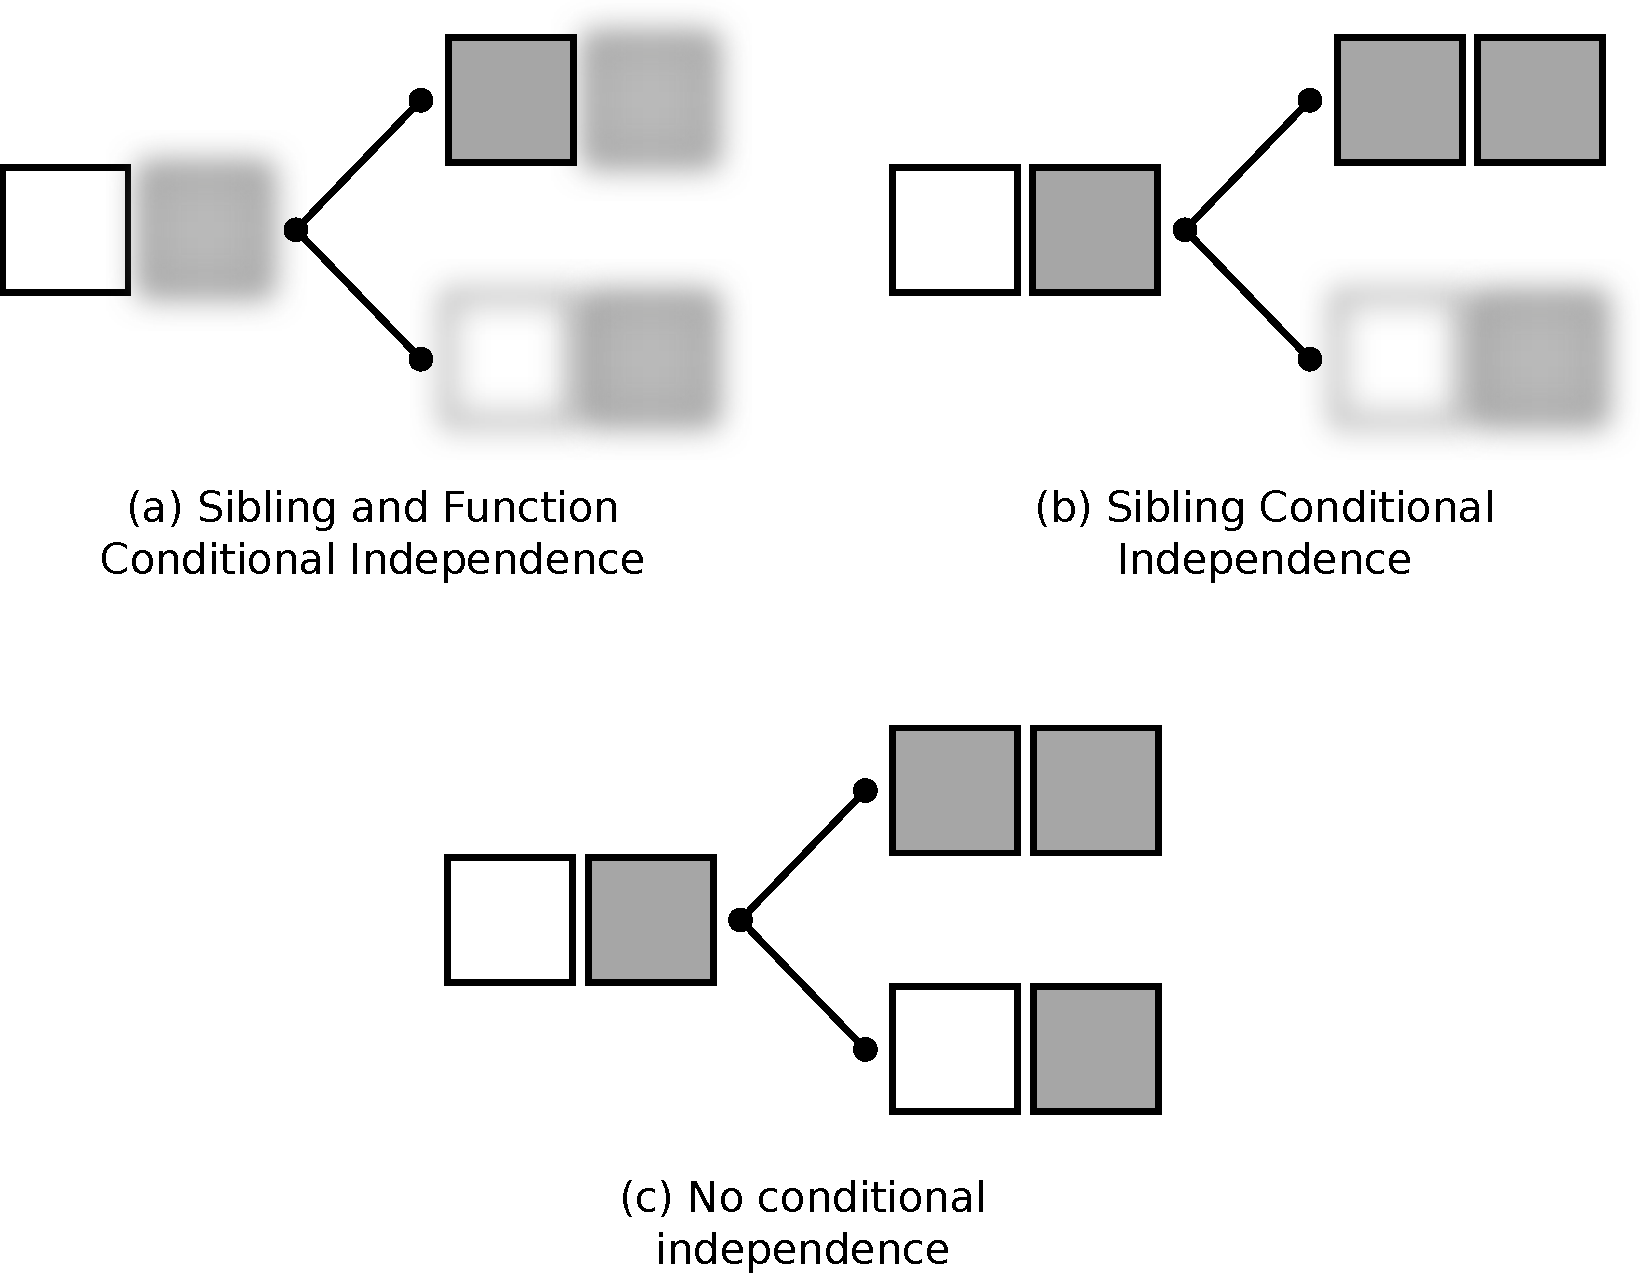
\includegraphics[width=.6\linewidth]{phylo-model-overview.pdf}
\end{figure}
}


\end{frame}

% ------------------------------------------------------------------------------
% ------------------------------------------------------------------------------
% ------------------------------------------------------------------------------
% ------------------------------------------------------------------------------
\section{Data}

\begin{frame}
	\usebeamertemplate{section intro}{}{}
	\textcolor{uscgold}{
		\Large {\bf Data} \vskip0.25em
		\large Phylogenetic trees and Experimental Annotations
	}
\end{frame}

\begin{frame}
	\frametitle{Data: Phylogenetic trees}
	
	
	
	Sample of annotations (first 10 in a single tree, Phosphoserine Phosphatase [PTHR10000])
	
	\small
	
	\begin{table}[ht]
		\centering
		\begin{tabular}{rrll}
			\toprule
			Internal id & Branch Length & type & ancestor \\ 
			\midrule
			AN0 &  & S & LUCA \\ 
			AN1 & 0.06 & S & Archaea-Eukaryota \\ 
			AN2 & 0.24 & S & Eukaryota \\ 
			AN3 & 0.44 & S & Unikonts \\ 
			AN4 & 0.42 & S & Opisthokonts \\ 
			AN6 & 0.68 & D &  \\ 
			AN9 & 0.79 & S & Amoebozoa \\ 
			AN10 & 0.18 & D &  \\ 
			AN15 & 0.57 & S & Dictyostelium \\ 
			AN18 & 0.52 & S & Alveolata-Stramenopiles \\ 
			\bottomrule
		\end{tabular}
	\end{table}
	
\end{frame}

\begin{frame}
	\frametitle{Data: Node type (events)}
	\begin{figure}
		\centering
		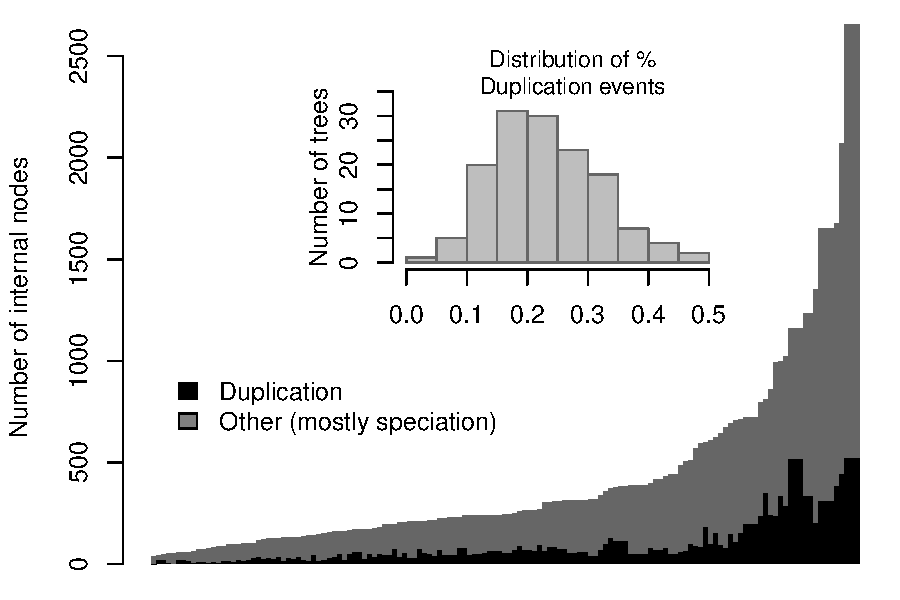
\includegraphics[width=.7\linewidth]{distribution-event-type.pdf}
	\end{figure}
\end{frame}

\begin{frame}
	\frametitle{Data: Annotations (example)}
	
	This is the first 10 of $\sim$ 400,000 experimental annotations used:
	
	\footnotesize
	\begin{table}[ht]
		\centering
		\begin{tabular}{rllll}
			\toprule
			& Family & Id & GO term & Qualifier \\ 
			\midrule
			1 & PTHR12345 & HUMAN$|$HGNC=15756$|$UniProtKB=Q9H190 & GO:0005546 &  \\ 
			2 & PTHR11361 & HUMAN$|$HGNC=7325$|$UniProtKB=P43246 & GO:0016887 & CONTRIBUTES\_TO \\ 
			3 & PTHR10782 & MOUSE$|$MGI=MGI=3040693$|$UniProtKB=Q6P1E1 & GO:0045582 &  \\ 
			4 & PTHR23086 & ARATH$|$TAIR=AT3G09920$|$UniProtKB=Q8L850 & GO:0006520 &  \\ 
			5 & PTHR32061 & RAT$|$RGD=619819$|$UniProtKB=Q9EPI6 & GO:0043197 &  \\ 
			6 & PTHR46870 & ARATH$|$TAIR=AT3G46870$|$UniProtKB=Q9STF9 & GO:1990825 &  \\ 
			7 & PTHR15204 & MOUSE$|$MGI=MGI=1919439$|$UniProtKB=Q9Z1R2 & GO:0045861 &  \\ 
			8 & PTHR22928 & DROME$|$FlyBase=FBgn0050085$|$UniProtKB=Q9XZ34 & GO:0030174 &  \\ 
			9 & PTHR35972 & HUMAN$|$HGNC=34401$|$UniProtKB=A2RU48 & GO:0005515 &  \\ 
			10 & PTHR10133 & DROME$|$FlyBase=FBgn0002905$|$UniProtKB=O18475 & GO:0097681 &  \\ 
			\bottomrule
		\end{tabular}
	\end{table}
\end{frame}

\begin{frame}
	\frametitle{Data: Experimental Annotations}
	\begin{figure}
		\centering
		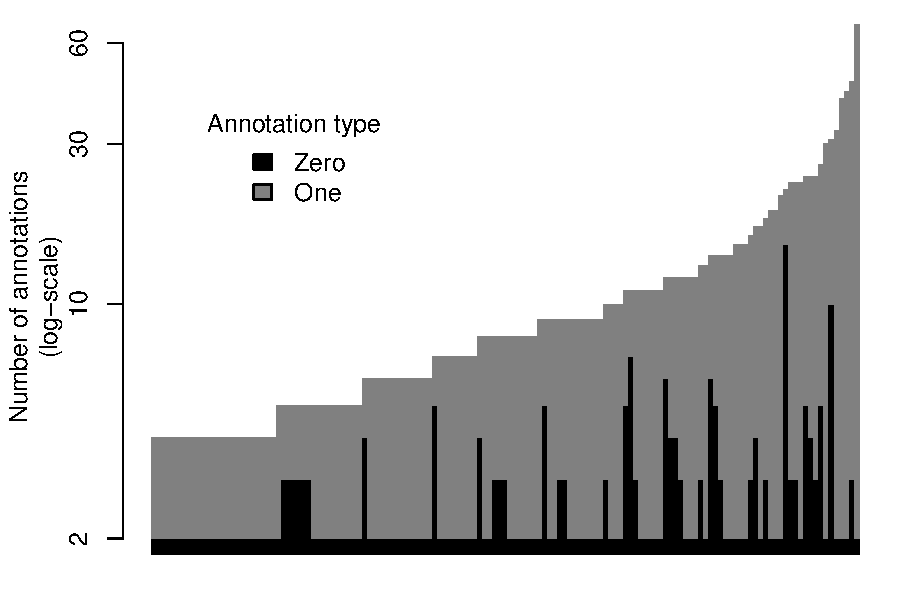
\includegraphics[width=.7\linewidth]{distribution-annotation-type.pdf}
	\end{figure}
\end{frame}


% ------------------------------------------------------------------------------
%\begin{frame}[t]
%\frametitle{Prediction with real data}
%
%\begin{minipage}{.39\linewidth}
%\begin{table}[ht]
%\centering
%\scalebox{0.7}{
%\begin{tabular}{ll*{2}{m{0.3\linewidth}<\centering}}
%  \toprule
% & & \multicolumn{2}{c}{Prior} \\
% & & Uniform & Beta  \\ 
%  \midrule
%  \multicolumn{2}{l}{Mislab. prob.} \\
%  & $\psi_0$ & 0.23 & 0.25 \\ 
%  & $\psi_1$ & 0.01 & 0.01 \\ 
%  \multicolumn{2}{l}{\textcolor<4->{usccardinal}{\textbf<4->{Gain/Loss at dupl.}}} \\
%  & $\mu_{d0}$ & 0.97 & 0.96 \\ 
%  & $\mu_{d1}$ & 0.52 & 0.58 \\ 
%  \multicolumn{2}{l}{\textcolor<4->{usccardinal}{\textbf<4->{Gain/Loss at spec.}}} \\
%  & $\mu_{s0}$ & 0.05 & 0.06 \\ 
%  & $\mu_{s1}$ & 0.01 & 0.02 \\ 
%  \multicolumn{2}{l}{Root node} \\
%  & $\pi$ & 0.81 & 0.45  \\ 
%\midrule 
%\multicolumn{2}{l}{Leave-one-out AUC} \\
%  & Mean & 0.69 & 0.67 \\
%  & Median & 0.81 & 0.75 \\
%   \bottomrule
%\end{tabular}
%}
%\caption{Parameter estimates using different priors.} 
%\end{table}
%%
%\end{minipage}
%\begin{minipage}{.59\linewidth}
%\begin{itemize}[<+->]
%\item 141 pooled functions (trees) with 7,388 genes with 0/1 annotations.
%\item Parameter estimates are actually probabilities.
%\item Data driven results (uninformative prior).
%\item \textcolor{usccardinal}{Biologically meaningful results.}
%\item Took about 5 minutes each.
%\end{itemize}
%\end{minipage}
%
%\end{frame}

\note[enumerate]{
\item The data used here corresponds to a subset of the trees.
\item Right now, the main criteria was: (1) must have at least one annotation
of each type, and (2) must not have large sets of siblings (this due to
numerical underflow issues, WIP)
}

\begin{frame}[t]
	\frametitle{Overview of Prediction Results}
	
	\begin{minipage}[t]{.55\linewidth}
		\vspace{-.5cm}
		\begin{table}
		\centering
		\scalebox{.64}{
%			\begin{tabular}{l*{4}{m{.22\linewidth}<\centering}}
			\begin{tabular}{%
					m{.24\linewidth}<\raggedright %
					>{\color<1>{usccardinal}}m{.24\linewidth}<\centering%
					>{\color<2>{usccardinal}}m{.24\linewidth}<\centering%
					>{\color<3>{usccardinal}}m{.24\linewidth}<\centering%
					>{\color<4>{usccardinal}}m{.24\linewidth}<\centering}
				\toprule
				& & \multicolumn{3}{c}{Type of Annotation} \\
				\cmidrule(r){3-5} %
					\phantom{\LARGE Cellular Component}& %
					\alt<1>{\LARGE Pooled}{Pooled} & %
					\alt<2>{\LARGE Molecular Function}{Molecular Function} & %
					\alt<3>{\LARGE Biological Process}{Biological Process} & %
					\alt<4>{\LARGE Cellular Comp.}{Cellular Component} \\ 
				\midrule
				\multicolumn{3}{l}{\hspace{-10pt}Mislabeling} \\
				$\psi_{01}$ & 0.23 & 0.18 & 0.09 & 0.66 \\ 
				$\psi_{10}$ & 0.01 & 0.01 & 0.01 & 0.33 \\ 
				\multicolumn{3}{l}{\hspace{-10pt}Duplication Events} \\
				$\mu_{d01}$ & 0.97 & 0.97 & \hlcAlt{3}{0.10} & 0.55 \\ 
				$\mu_{d10}$ & 0.52 & 0.51 & \hlcAlt{3}{0.03} & 0.56 \\ 
				\multicolumn{3}{l}{\hspace{-10pt}Speciation Events} \\
				$\mu_{s01}$ & 0.05 & 0.05 & 0.05 & 0.37 \\ 
				$\mu_{s10}$ & 0.01 & 0.01 & 0.02 & 0.37 \\ 
				\multicolumn{3}{l}{\hspace{-10pt}Root node} \\
				$\pi$ & 0.79 & 0.71 & 0.88 & 0.52 \\ \midrule
				Trees & 141 & 74 & 45 & 22 \\ 
				\multicolumn{3}{l}{\hspace{-10pt}Accuracy under the by-aspect model} \\
				AUC & - & \hlcAlt{2}{0.77} & \hlcAlt{3}{0.83} & 0.53 \\ 
				MAE & - & \hlcAlt{2}{0.34} & \hlcAlt{3}{0.26} & 0.50 \\ 
				\multicolumn{3}{l}{\hspace{-10pt}Accuracy under the pooled-data model} \\
				AUC & - & \hlcAlt{2}{0.77} & 0.75 & 0.75 \\ 
				MAE & - & \hlcAlt{2}{0.35} & 0.34 & 0.37 \\ 
				\bottomrule
		\end{tabular}}
		%\caption[Parameter estimates comparing pooled-data vs by-type]{MCMC estimates for experimentally annotated trees. The first column shows the estimates under the pooled-data model in \ref{tab:pooled-experimentally-annotated}, while the following three columns report the estimates obtained when fitting the model using a pooled-data approach, but doing so by type of annotation. Readers should be aware that the estimation process of the fourth column, \textit{cellular component}, did not fully converge, likely due to sparsity of annotations within that category.}
		\label{tab:by-aspect-estimates}
	\end{table}
	\end{minipage}
\hfill
\begin{minipage}[t]{.44\linewidth}
	Previously, joint estimates out-performed one-at-a-time\pause
	\begin{itemize}[<+->]
		\item \textbf{Molecular Function} No change.
		\item \textbf{Biological Process} Significantly better.
		\item \textbf{Cellular Component} does not converge.
	\end{itemize}
\end{minipage}
	


\end{frame}

\section{abc}

\begin{frame}[t]
	\frametitle{Example 1: Good quality prediction}
	
\begin{minipage}[m]{.3\linewidth}
	\small
%	The AUC for this analysis is 0.91 and the Mean Absolute Error is 0.34
	\textbf{MAE:} 0.34 \\
	\textbf{AUC:} 0.91 \\
	\textbf{Type:} Molecular Function\\
	\textbf{Name:} 2'-5'-oligoadenylate synthetase activity\\
	\textbf{Desc:}  \href{http://amigo.geneontology.org/amigo/term/GO:0001730}{\alert{GO:0001730}} involved in the process of cellular antiviral activity (wiki on \href{https://en.wikipedia.org/wiki/Interferon}{\alert{interferon}}).
\end{minipage}
\begin{minipage}[m]{.65\linewidth}
	\def\tmpwdth{.9\linewidth}
	\mode<beamer>{
		\centering
		\only<1>{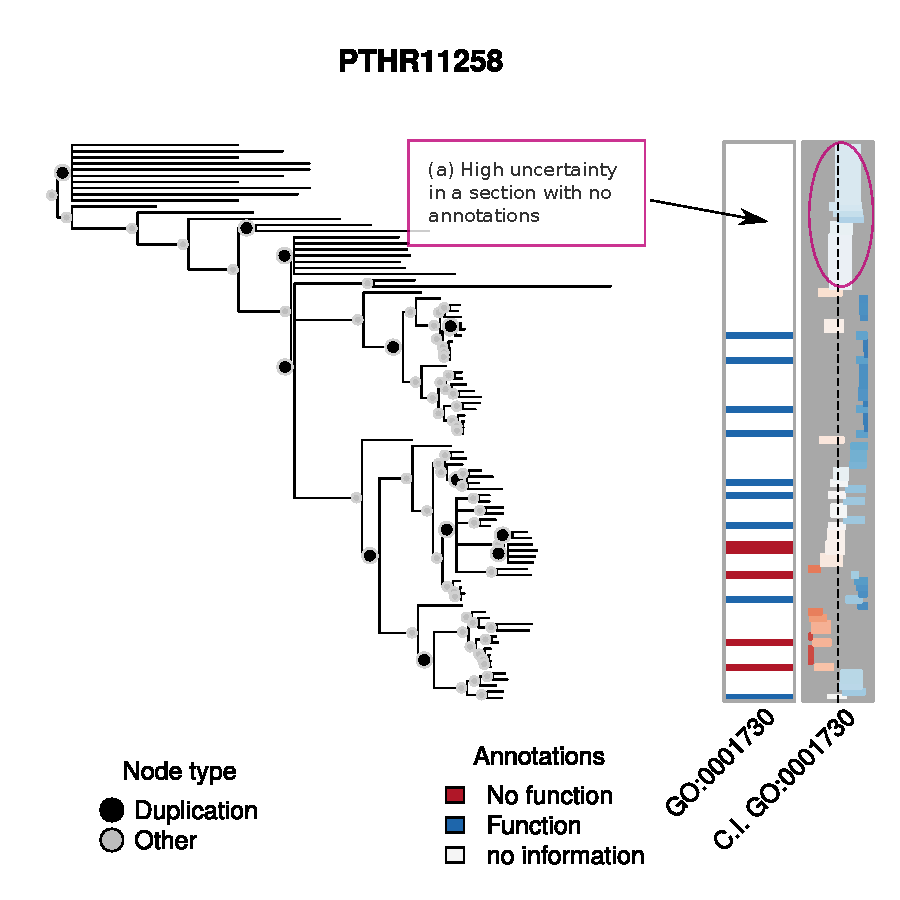
\includegraphics[width=\tmpwdth, clip, trim={0 0 0 2cm}]{example-trees-good1-loo-annotated-1.pdf}}\only<2>{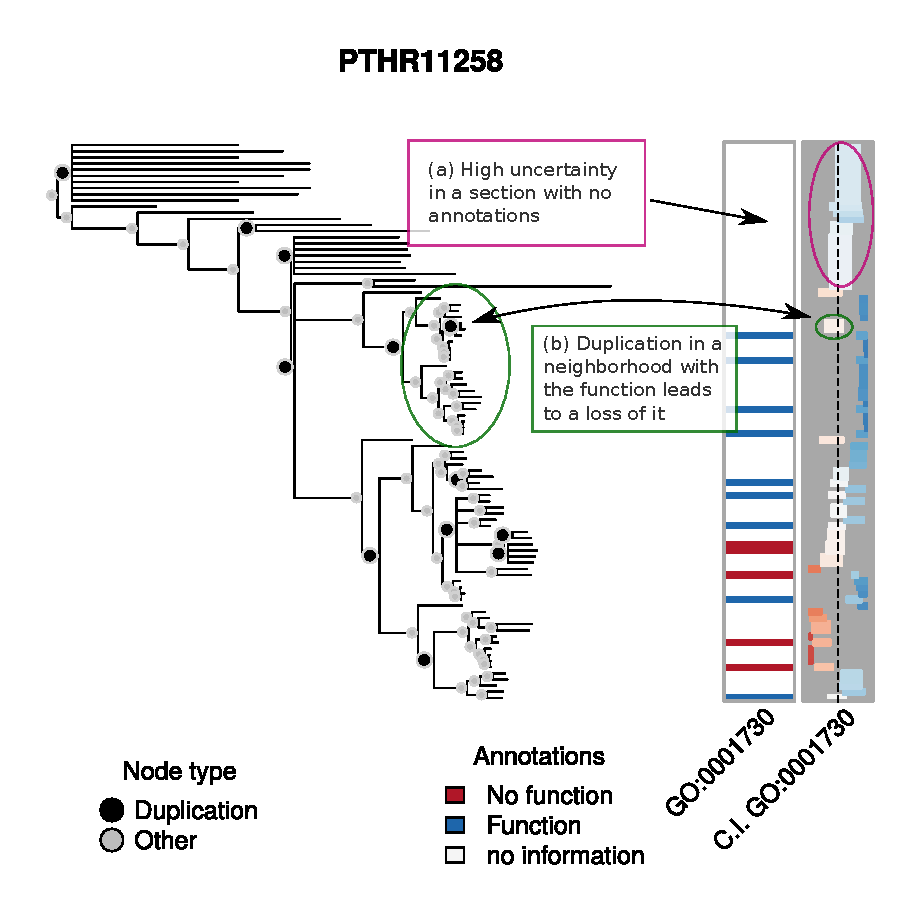
\includegraphics[width=\tmpwdth, clip, trim={0 0 0 2cm}]{example-trees-good1-loo-annotated-2.pdf}}\only<3>{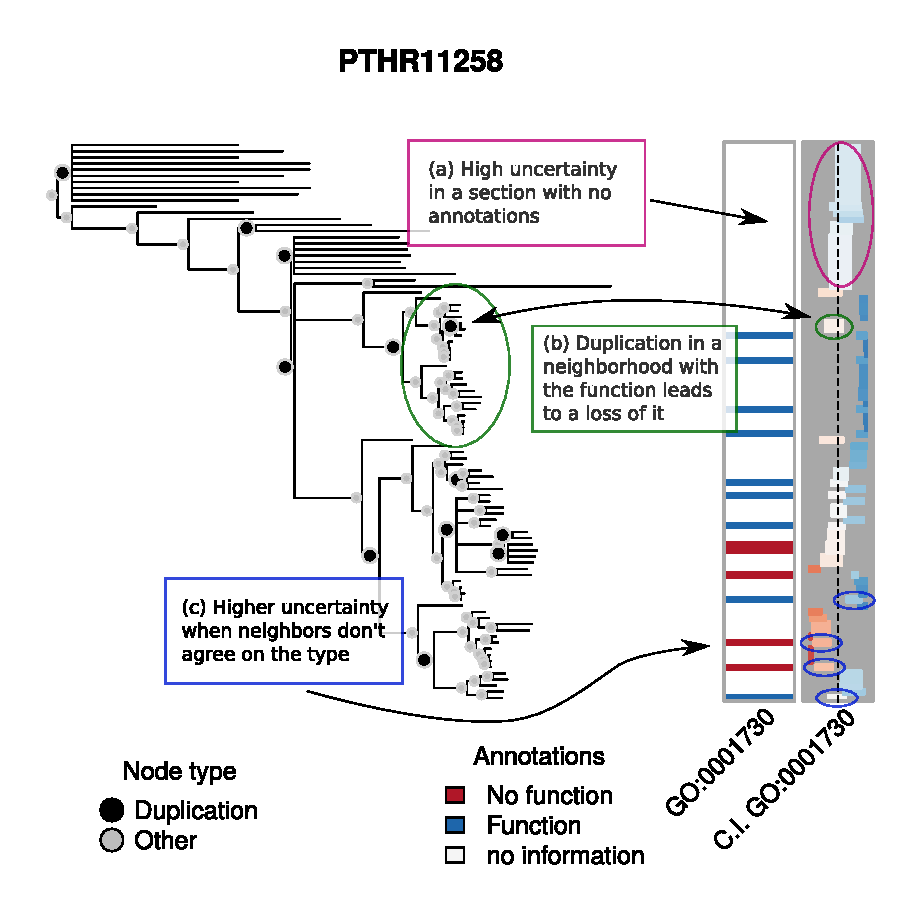
\includegraphics[width=\tmpwdth, clip, trim={0 0 0 2cm}]{example-trees-good1-loo-annotated.pdf}}
	}
	
	\mode<handout>{
		\centering
		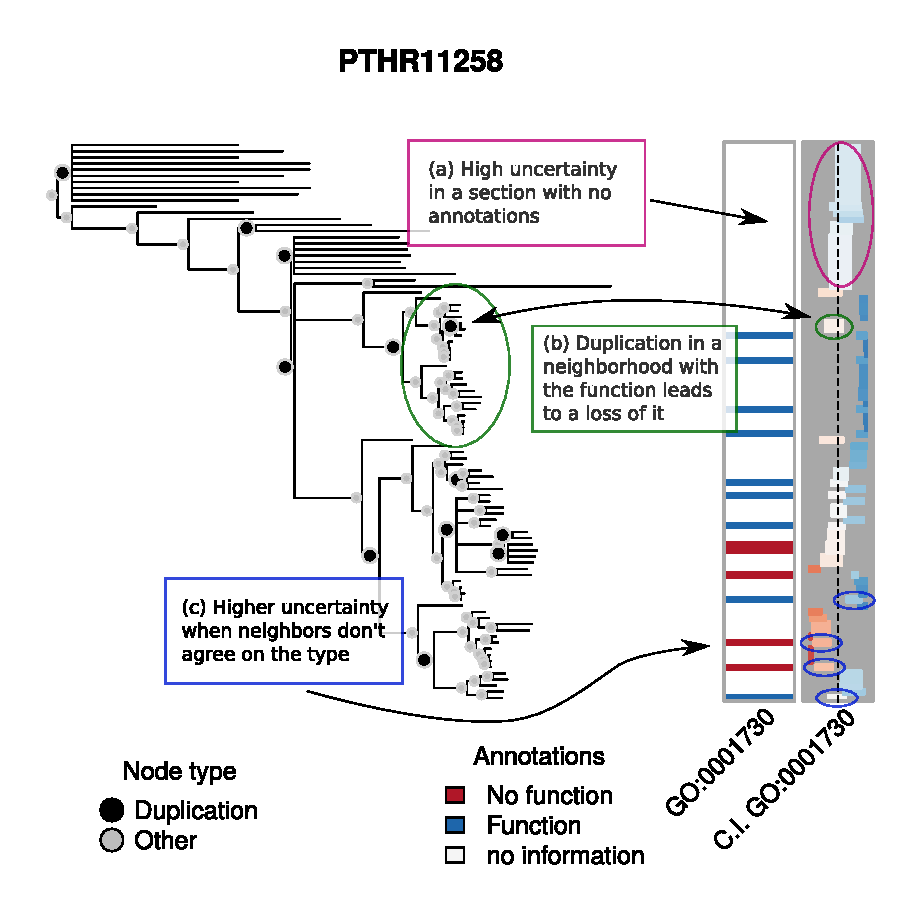
\includegraphics[width=\tmpwdth, clip, trim={0 0 0 2cm}]{example-trees-good1-loo-annotated.pdf}
	}
	
\end{minipage}
\end{frame}


\begin{frame}[t]
	\frametitle{Example 2: Bad quality prediction}
	
	\begin{minipage}[m]{.3\linewidth}
		\small
		%	The AUC for this analysis is 0.91 and the Mean Absolute Error is 0.34
		\textbf{MAE:} 0.52 \\
		\textbf{AUC:} 0.33 \\
		\textbf{Type:} Molecular Function\\
		\textbf{Name:} mannosyl-oligosaccharide 1,2-alpha-mannosidase activity\\
		\textbf{Desc:}  \href{http://amigo.geneontology.org/amigo/term/GO:0004571}{\alert{GO:0004571}} involved in synthesis of glycoproteins (\href{https://en.wikipedia.org/wiki/Mannosyl-oligosaccharide_1,2-alpha-mannosidase}{\alert{wiki}} and \href{https://en.wikipedia.org/wiki/Glycoprotein}{\alert{examples}}).
	\end{minipage}
	\begin{minipage}[m]{.65\linewidth}
		\def\tmpwdth{.9\linewidth}
		\mode<beamer>{
			\centering
			\only<1>{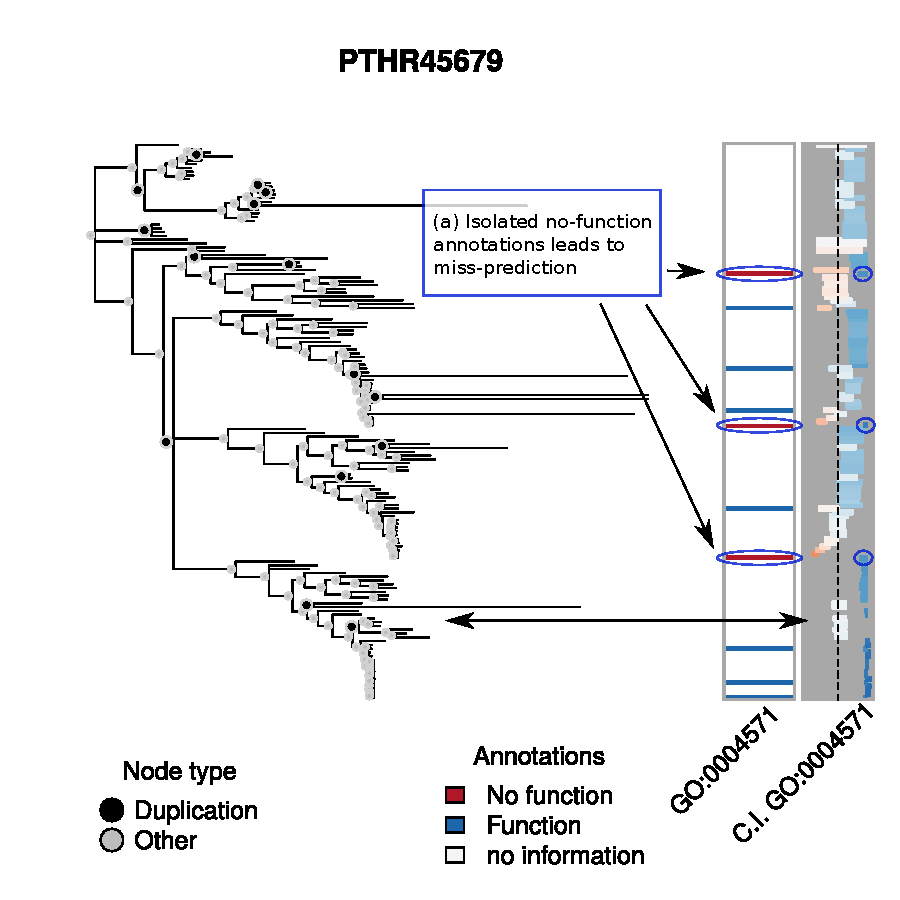
\includegraphics[width=\tmpwdth, clip, trim={0 0 0 2cm}]{example-trees-bad1-loo-annotated-1.pdf}}\only<2>{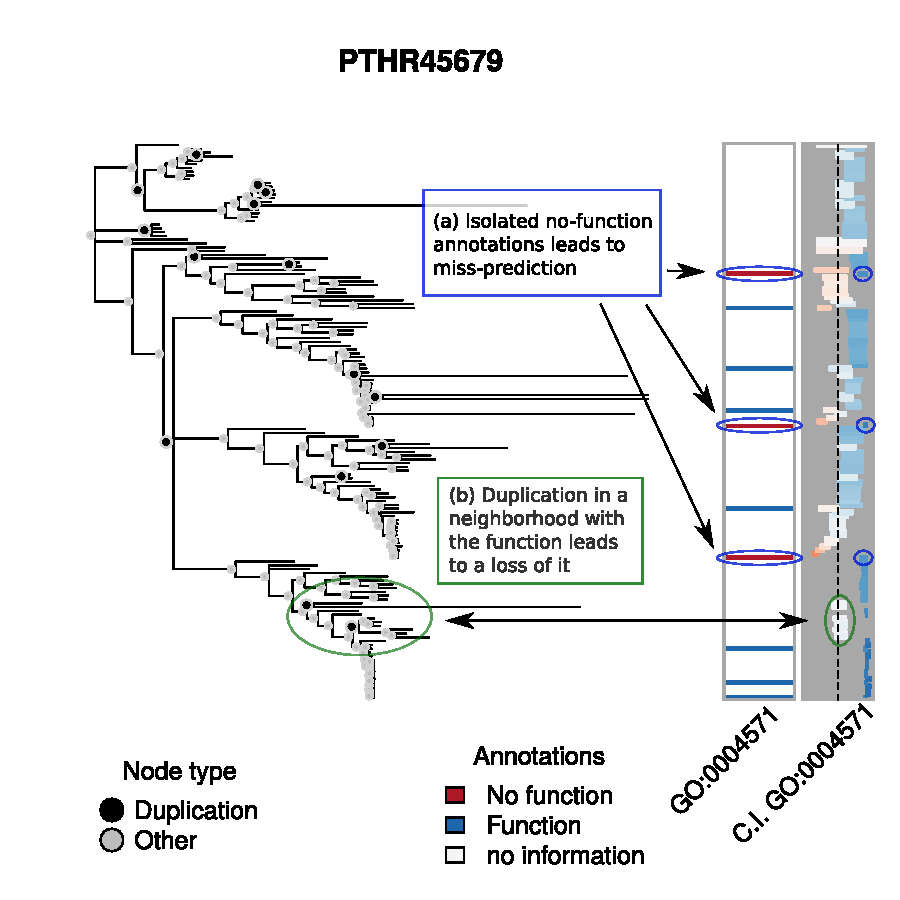
\includegraphics[width=\tmpwdth, clip, trim={0 0 0 2cm}]{example-trees-bad1-loo-annotated.pdf}}
		}
		
		\mode<handout>{
			\centering
			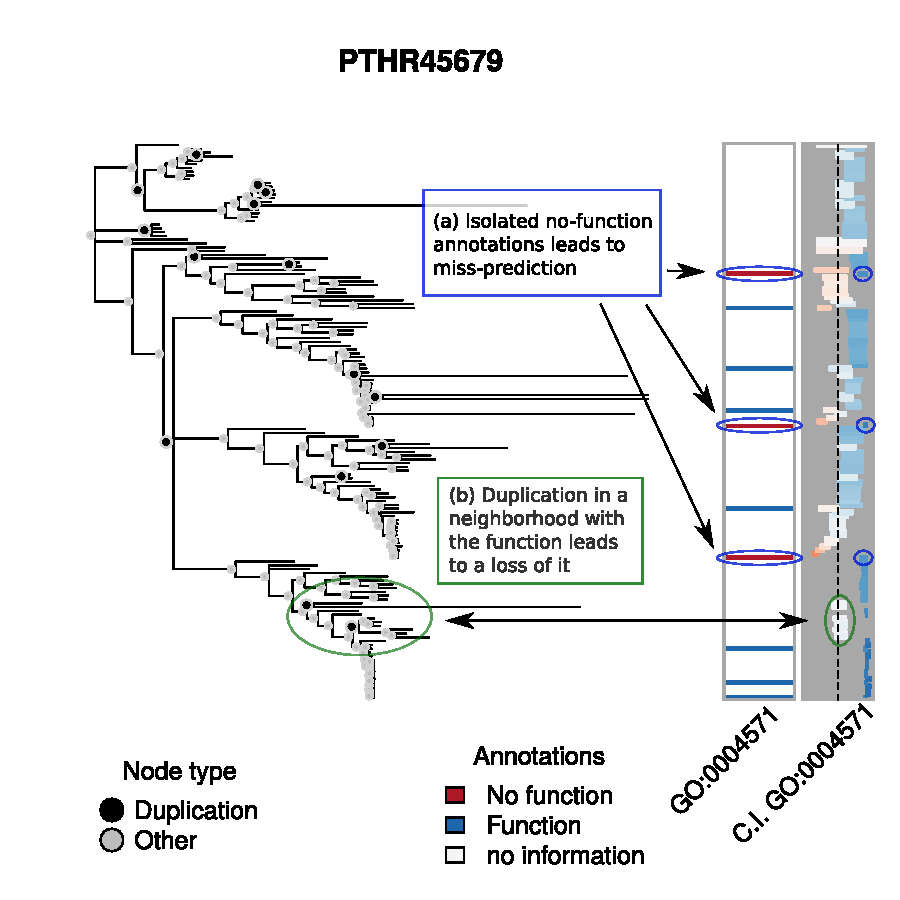
\includegraphics[width=\tmpwdth, clip, trim={0 0 0 2cm}]{example-trees-bad1-loo-annotated.pdf}
		}
		
	\end{minipage}
	
	
\end{frame}

% ------------------------------------------------------------------------------
\begin{frame}[t]
	\frametitle{Future Research: phylogenetic models}
	
	Imagine that we have 3 functions (rows) and that each node has 2 siblings (columns)
	
	\mode<beamer>{
		\begin{table}
			\begin{tabular}{llcc}
				\toprule
				& & \multicolumn{2}{c}{\bf Transitions to} \\
				& & Case 1 & Case 2 \\ \cmidrule(r){3-4}
				\multicolumn{2}{r}{\textbf{Parent} $\begin{array}{c}\mbox{A} \\ \mbox{B} \\ \mbox{C}\end{array}\left[\begin{array}{c}0 \\ 1 \\ 1\end{array}\right]$} & 
				$\left[\begin{array}{cc} %
				0 & \nhlc{1-2}{1}\hlc{3-5}{1}\nhlc{6-}{1} \\ %
				1 & \nhlc{1-3}{0}\hlc{4-5}{0}\nhlc{6-}{0} \\ %
				1 & \nhlc{1-3}{0}\hlc{4}{1}\nhlc{5-}{1} %
				\end{array}\right]$ & 
				$\left[\begin{array}{cc} %
				0 & \nhlc{-2}{1}\nhlc{4}{1}\hlc{3}{1}\hlc{5}{1}\nhlc{6-}{1} \\ %
				\nhlc{-5}{1}\hlc{6}{1}\nhlc{7-}{1} & \nhlc{-4}{0}\hlc{5}{0}\nhlc{6-}{0}\\ %
				\nhlc{-4}{0}\hlc{5}{0}\nhlc{6-}{0} & \nhlc{1-5}{1}\hlc{6}{1}\nhlc{7-}{1}%
				\end{array}\right]$ \pause \\ \midrule 
				\multicolumn{3}{l}{\textbf{Sufficient statistics}} \pause \\ 
				& \# Gains (Neofunctionalization) & 1 & 1 \pause \\
				& Only one offspring changes (yes/no) & 1 & 0 \pause \\
				& \# Changes (gain+loss) & 2 & 3 \pause \\
				& Subfunctionalization (yes/no) & 0 & 1 \\ \bottomrule
			\end{tabular}
		\end{table}
	}
	\mode<handout>{
		\begin{table}
			\begin{tabular}{llcc}
				\toprule
				& & \multicolumn{2}{c}{\bf Transitions to} \\
				& & Case 1 & Case 2 \\ \cmidrule(r){3-4}
				\multicolumn{2}{r}{\textbf{Parent} $\begin{array}{c}\mbox{A} \\ \mbox{B} \\ \mbox{C}\end{array}\left[\begin{array}{c}0 \\ 1 \\ 1\end{array}\right]$} & 
				$\left[\begin{array}{cc} %
				0 & 1 \\ %
				1 & 0 \\ %
				1 & 1 %
				\end{array}\right]$ & 
				$\left[\begin{array}{cc} %
				0 & 1 \\ %
				1 & 0\\ %
				0 & 1%
				\end{array}\right]$ \\ \midrule 
				\multicolumn{3}{l}{\textbf{Sufficient statistics}} \\ 
				& \# Neofunctionalizations & 1 & 1  \\
				& Only one offspring changes (yes/no) & 1 & 0 \\
				& \# Changes (gain+loss) & 2 & 3 \\
				& Subfunctionalizations (yes/no) & 0 & 1 \\ \bottomrule
			\end{tabular}
		\end{table}
	}
	
	\pause
	Modeling the full Markov transition matrix would take $2^3 \times 2^6 = 512$ parameters.
	
\end{frame}


% ------------------------------------------------------------------------------
\begin{frame}[t]
\frametitle{Paper 1: On the prediction of gene functions using phylogenetic trees}

{\bf \large Key takeaways}
\begin{beamercolorbox}[dp=1ex]{conclusions}
\begin{itemize}
\item A parsimonious model for predicting gene functions using phylogenetics.
\item Computationally scalable. SIFTER (our benchmark)
would take about 66 years (yes, years) to estimate a model for 100 families
of size 300, we take about 5 minutes.
\item Meaningful biological results.
\item Preliminary accuracy results comparable to state-of-the-art phylo-based models.
\end{itemize}
\end{beamercolorbox}\pause

{\bf \large Challenges}
\begin{beamercolorbox}[dp=1ex]{conclusions}
\begin{itemize}
\item Offspring are conditional independent on their parent and\pause{}
\item Functions evolve independently. \hyperlink{duplicationvsspeciation}{\beamergotobutton{more}}
\end{itemize}
\end{beamercolorbox}

\end{frame}


% ------------------------------------------------------------------------------
\section{Chapter 3: Discrete Exponential Family Models}
% \frame{\frametitle{Contents}\tableofcontents}

\begin{frame}[t]
	\usebeamertemplate{section intro}{}{}
	\textcolor{uscgold}{
		\Large {\bf Discrete Exponential Family Models} \vskip0.25em
%		\large \textit{Joint with}: Andrew Slaughter and Kayla de la Haye
	}
\end{frame}

\begin{frame}[t]

\frametitle{Canonical Equation}

\begin{figure}
	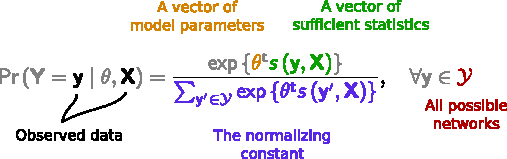
\includegraphics[width=.7\linewidth]{parts-of-ergm.pdf}
\end{figure}

%\begin{center}
%\begin{equation*}
%\Prcond{\Graph = \graph}{X = x} = \frac{%
%\exp{\t{\beta}\s{\graph, x}} %
%}{%
%\sum_{\graph'\in\GRAPH} \exp{\t{\beta}\s{\graph', x}} %
%},\quad \forall \graph\in\GRAPH
%\end{equation*}
%\end{center}

\vfill

\begin{minipage}[m]{.45\linewidth}

\begin{itemize}
	\item<2-> For any array of size $(n\times m)$, there are $2^{(n\times m)}$ possible arrangements.
	\item<3-> Focused on vector of sufficient statistics $\s{\graph,x}$ (not the edges themselves) \uncover<4->{\textbf{e.g.}\\Two Bernoulli, a.k.a. Erd\H{o}s-R\'enyi, random graphs}
\end{itemize}
\end{minipage}\hfill
\begin{minipage}[m]{.45\linewidth}
	\begin{figure}[!htbp]
		\centering
		\includegraphics<4->[width=.8\linewidth,clip,trim={.5cm .5cm .5cm .5cm}]{ring-and-kite.pdf}
%		\caption[Simple graphs: A ring and a Kite]{Although these two networks may look very different, \textit{a ring} and \textit{a kite}, under the Bernoulli, also known as Erd\H{o}s-R\'enyi, random graph model, both are equally likely, as the only sufficient statistic for this model is the number of observed ties, which is five in both cases.}
		\label{fig:ring-and-kite}
	\end{figure}
\end{minipage}


\end{frame}


\begin{frame}
\frametitle{Asymptotic Behavior of ERGMs}

\begin{itemize}
\item In the case that $s_l = \s{\graph, x}$ is on the boundary: $s_l \to \pm\infty$
\item Since the support space of $\s{\graph, x}\in\SUFF$ is bounded, e.g. \# edges $\in [0,n\times (n - 1)]$, we have: 

\begin{equation*}
\lim_{\theta_l\to\infty}\loglik{\theta}, \quad %
\lim_{\theta_l\to\infty}\nabla\loglik{\theta}, \quad %
\lim_{\theta_l\to\infty}\mathbf{H}\left(\theta\right)
\end{equation*}
log-likelihood, its gradient, and hessian are finite.
\item The direct implication is that, while $\s{\graph, x}$ is on the boundary, the MLE for the other statistics exists.\footnote{\cite{Handcock2003} briefly mentions this}
\item All equations ultimately involve realizations of $\s{\graph', x}$ that equal $s_l$, relevant in: Simulations, Bootstrapping, etc.
\end{itemize}


\end{frame}

\begin{frame}
\frametitle{Conditional Distribution}

\begin{equation*}
\Prcond{\sufstats{\Graph}_k = s_k}{\sufstats{\Graph}_l = s_l, \theta} = %
\frac{%
	\exp{\transpose{\theta}_{-l}\sufstats{\graph}_{-l}}
}{%
	\sum_{\graph': \sufstats{\graph'}_l = \sufstats{\graph}_l}\exp{\transpose{\theta}_{-l}\sufstats{\graph'}_{-l}}
}\tag{3.5}
\end{equation*}


\end{frame}

% ------------------------------------------------------------------------------
\section{Paper 2: Exponential Random Graph Models for Small Networks}
% \frame{\frametitle{Contents}\tableofcontents}

\begin{frame}[t]
\usebeamertemplate{section intro}{}{}
\textcolor{uscgold}{
\Large {\bf Exponential Random Graph Models for Small Networks} \vskip0.25em
\large \textit{Joint with}: Andrew Slaughter and Kayla de la Haye
}
\end{frame}

\begin{frame}
\frametitle{What are Exponential Random Graph Models}

Exponential Family Random Graph Models, aka \alert{ERGMs} are:\pause

\begin{itemize}[<+->]
\item Statistical models of (social) networks
\item In simple terms: statistical inference on what network patterns/structures/motifs
govern social networks
\begin{figure}
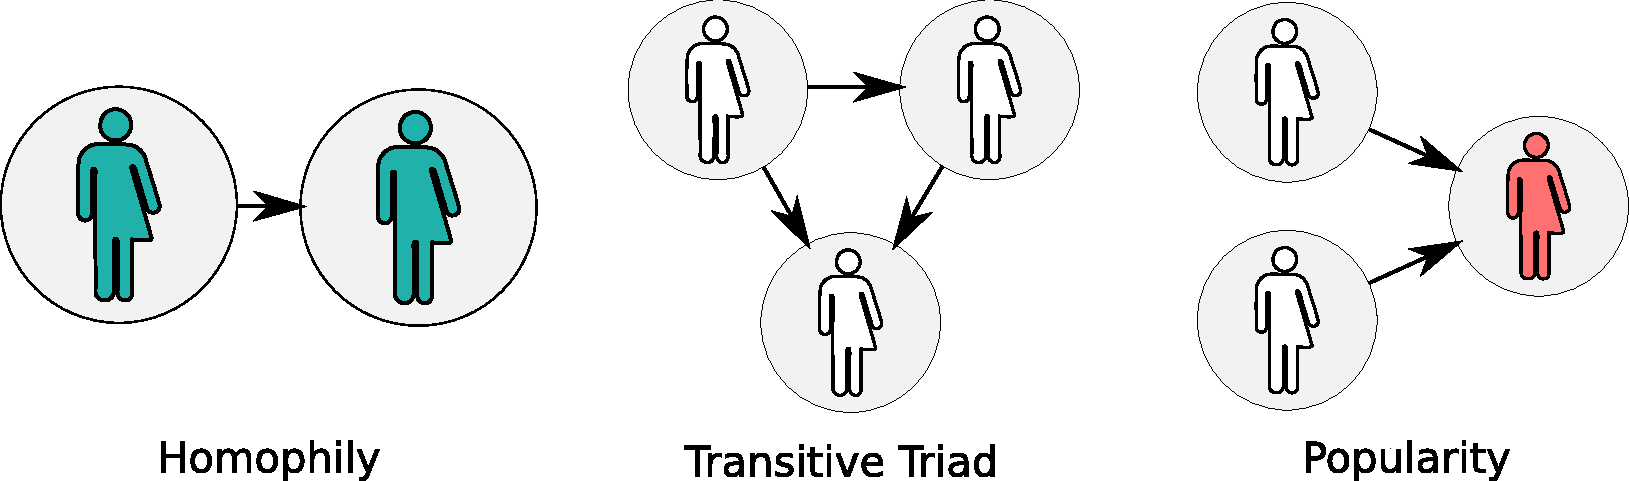
\includegraphics[width=.6\linewidth]{friendly-terms.pdf}
\end{figure}
\end{itemize}

\end{frame}

% ------------------------------------------------------------------------------
\begin{frame}[label=ergmterms]

{\bf\color{suffstat} Sufficient statistics} have various forms

\def\fig1width{.45\linewidth}
\begin{figure}[!htbp]
	\centering
	\begin{tabular}{m{.2\linewidth}<\centering m{.4\linewidth}<\raggedright}
		\toprule Representation & Description  \\ \midrule
		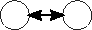
\includegraphics[width=\fig1width]{mutual.pdf} & Mutual Ties (Reciprocity)\linebreak[4]$\sum_{i\neq j}y_{ij}y_{ji}$  \\
		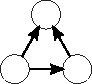
\includegraphics[width=\fig1width]{ttriad.pdf} & Transitive Triad (Balance)\linebreak[4]$\sum_{i\neq j\neq k}y_{ij}y_{jk}y_{ik}$  \\
		
\includegraphics[width=\fig1width]{homophily.pdf} & Homophily\linebreak[4]$\sum_{i\neq j}y_{ij}\mathbf{1}\left(x_i=x_j\right)$ \\
		
\includegraphics[width=\fig1width]{nodeicov2.pdf} & Attribute-receiver effect \linebreak[4]$\sum_{i\neq j}y_{ij}x_j$ \\
		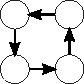
\includegraphics[width=\fig1width]{fourcycle.pdf} & Four Cycle\linebreak[4]$\sum_{i\neq j \neq k \neq l}y_{ij}y_{jk}y_{kl}y_{li}$  \\
		\bottomrule
	\end{tabular}
	\caption[Example of Graph Sufficient Statistics]{Besides of the common edge count statistic (number of ties in a graph), ERGMs allow measuring other more complex structures that can be captured as sufficient statistics. }
	\label{fig:ergm-structs}
\end{figure}

% \vfill\hfill \hyperlink{ergmeq}{\beamerreturnbutton{go back}}
\end{frame}

% % ------------------------------------------------------------------------------
% \begin{frame}
% \frametitle{ERGMs for Small Networks}
% 
% From the methodological point of view, current methods are great, but:\pause
% 
% \begin{itemize}
% \item Possible accuracy issues (error rates)\pause
% \item Prone to degeneracy problems (sampling and existence of MLE)\pause
% \item It is not MLE...
% \end{itemize}
% 
% \end{frame}

% Simulation study -------------------------------------------------------------

\begin{frame}[t]
	\frametitle{Simulation Study}

	\begin{minipage}[t]{.3\linewidth}
		\begin{enumerate}
			\item \alert{\bf Higher convergence rate}
		\end{enumerate}
	\end{minipage}
\vfill\hfill\begin{minipage}[t]{.65\linewidth}\vspace{-.75cm}
	\begin{figure}
	\centering
		%\caption[Distribution of Converged and Non-converged Fits]{\label{fig:failed}Distribution of the average sufficient statistics per sample. Since samples can contain networks of sizes four and five, we have re-scaled the sufficient statistics counts by each network size's corresponding maximum value so these range from zero to one. Most of the cases in which methods failed to converge happened in scenarios where either all the graphs in the sample were fully connected or there was no transitive triad; exactly the cases that we excluded for the reminder of the analysis.}
		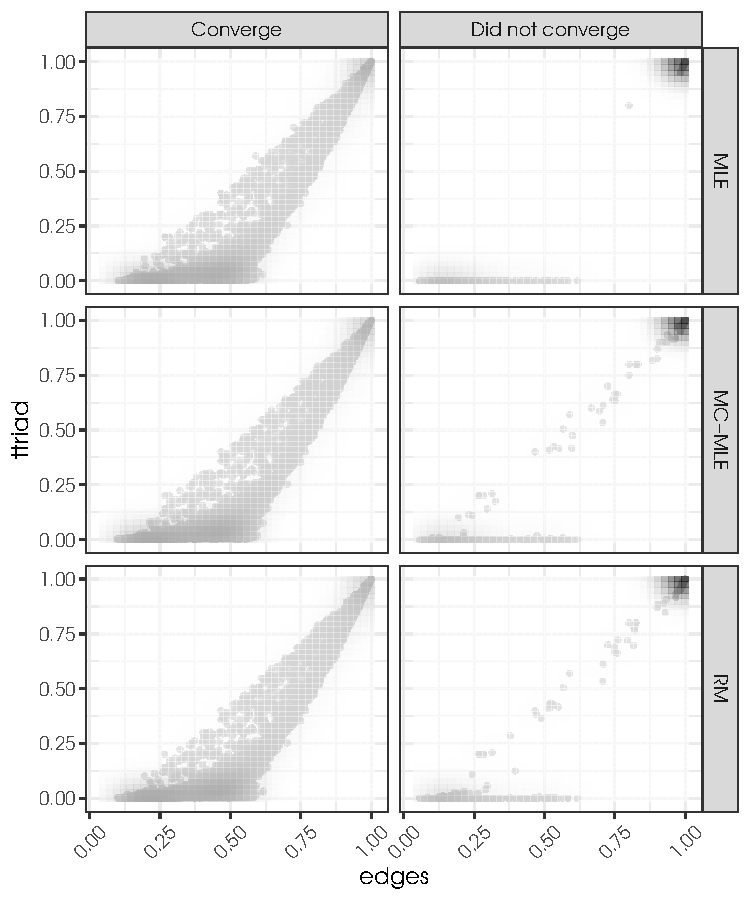
\includegraphics[width=.9\linewidth]{failed.pdf}
	\end{figure}
	\end{minipage}
\end{frame}

\begin{frame}[t, label=ergmitoexperiment]
	\frametitle{Simulation Study}

	\begin{minipage}[t]{.3\linewidth}
		\begin{enumerate}
			\item Higher convergence rate
			\item \alert{\bf Smaller Bias}
		\end{enumerate}
	\end{minipage}
\vfill\hfill\begin{minipage}[t]{.65\linewidth}\vspace{-.75cm}
		\begin{table}
		\centering
		\begin{tabular}{rccc}
			\toprule
			& MLE & MC-MLE & RM \\ 
			\midrule
			edges & [0.27, 0.36] & [1.23, 1.65] & [0.55, 1.54] \\ 
			ttriads & [-0.05, -0.03] & [-0.22, -0.16] & [-0.15, 0.48] \\ 
			\bottomrule
		\end{tabular}
%		\caption[Empirical Biases per Method]{\label{tab:empirical-bias-sim}Empirical bias. Each cell shows the 95\% confidence interval of each methods' empirical bias.} 
	\end{table}

\hfill\hyperlink{ergmito-bias}{\beamergotobutton{alt take}}
	\end{minipage}
\end{frame}

\begin{frame}[t]
	\frametitle{Simulation Study}
	
	\begin{minipage}[t]{.3\linewidth}
		\begin{enumerate}
			\item Higher convergence rate
			\item Smaller Bias
			\item \alert{\bf Higher power}
		\end{enumerate}
	\end{minipage}
\hfill\begin{minipage}[t]{.65\linewidth}%\vspace{-.75cm}
		\begin{figure}
			\centering
			%		\caption[Empirical Power by Sample and Effect Size]{\label{fig:power}Empirical power by dataset size and effect size (the later considering only magnitude), for ERGM and \ergmito{} estimation methods. Power increases for both MC-MLE (ERGM) and MLE (\ergmito{}) with increases in the size of the dataset and effect size. There are indistinguishable differences in power between the two estimation methods.}
			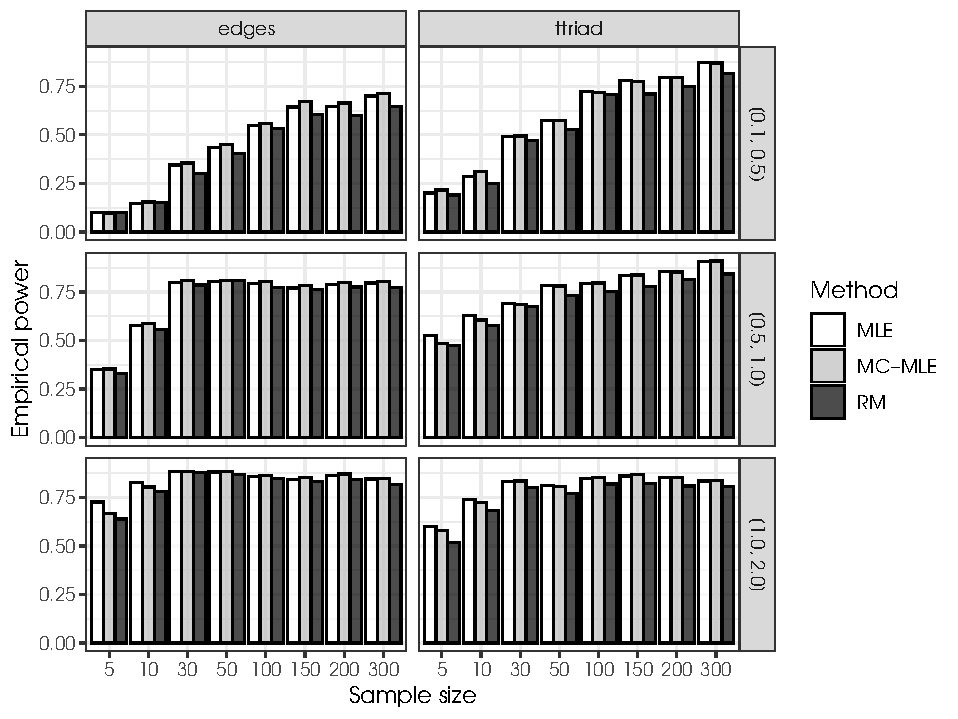
\includegraphics[width=.95\linewidth]{power.pdf}
		\end{figure}
	\end{minipage}
\end{frame}

\begin{frame}[t]
	\frametitle{Simulation Study}
	
	\begin{minipage}[t]{.3\linewidth}
		\begin{enumerate}
			\item Higher convergence rate
			\item Smaller Bias
			\item Higher power
			\item \alert{\bf Smaller Type I Error}
		\end{enumerate}
	\end{minipage}
\hfill\begin{minipage}[t]{.65\linewidth}%\vspace{-.75cm}
		\begin{table}
			\centering\small
			\begin{tabular}{*{2}{m{.1\linewidth}<\centering}*{5}{c}}
				\toprule & & \multicolumn{3}{c}{P(Type I error)} & \multicolumn{2}{c}{$\chi^2$ (vs MLE)}\\ \cmidrule(r){3-5} \cmidrule(r){6-7}
				Sample size & N. Sims. & MLE & MC-MLE & RM & MC-MLE & RM \\ 
				\midrule
				5 & 4,325 & 0.066 & 0.086 & 0.086 & 11.36 *** & 11.36 *** \\ 
				10 & 4,677 & 0.063 & 0.078 & 0.073 & 8.44 *** & 3.73 * \\ 
				15 & 4,818 & 0.060 & 0.072 & 0.063 & 5.50 ** & 0.41  \\ 
				20 & 4,889 & 0.054 & 0.065 & 0.061 & 5.30 ** & 2.05  \\ 
				30 & 4,946 & 0.053 & 0.059 & 0.055 & 1.60  & 0.07  \\ 
				50 & 4,987 & 0.053 & 0.055 & 0.047 & 0.16  & 1.67  \\ 
				100 & 4,999 & 0.054 & 0.054 & 0.050 & 0.00  & 0.81  \\ 
				\bottomrule
			\end{tabular}
			%		\caption[Empirical Type I Error Rates]{\label{tab:typeI}Empirical Type I error rates. The $\chi^2$ statistic is from a 2-sample test for equality of proportions, and the significance levels are given by *** $p < 0.01$, ** $p < 0.05$, and * $p < 0.10$.} 
		\end{table}
	\end{minipage}
\end{frame}

\begin{frame}[t]
	\frametitle{Simulation Study}
	
	\begin{minipage}[t]{.3\linewidth}
		\begin{enumerate}
			\item Higher convergence rate
			\item Smaller Bias
			\item Higher power
			\item Smaller Type I Error
			\item \alert{\bf Elapsed time}
		\end{enumerate}
	\end{minipage}
\hfill\begin{minipage}[t]{.65\linewidth}%\vspace{-.75cm}
		\begin{figure}
			\centering
			%	\caption[Distribution of Elapsed Time]{\label{fig:elapsedtime}Distribution of elapsed time (in seconds) for the estimation process for MC-MLE (ERGM) versus MLE (using \ergmito{}). Overall, the MLE implementation is orders of magnitude faster compared to the time required by the MC-MLE implementation to do the parameter estimation.}
			\small
			\def\svgwidth{.95\linewidth}
			\input{fig/time.pdf_tex}
		\end{figure}
	\end{minipage}
\end{frame}

% ------------------------------------------------------------------------------



\begin{frame}
	% latex table generated in R 3.6.3 by xtable 1.8-4 package
	% Mon Apr 27 23:32:51 2020
	\begin{table}[!htbp]
		\centering
		\begin{tabular}{*{3}{c}*{3}{m{.15\linewidth}<\centering}}
			\toprule
			(1) & (2) & (3) & (4) & (5) & (6) \\
			Size ($n$) & edges & ttriads & $\text{edges}\times\isone{n = 5}$ & $\text{ttriads}\times\isone{n = 5}$ & $\text{edges}\times\log{1/n}$ \\ 
			\midrule
			4 &  10 &  14 &   0 &   0 & -13.86 \\ 
			4 &   6 &   2 &   0 &   0 & -8.32 \\ 
			4 &   4 &   0 &   0 &   0 & -5.55 \\ 
			5 &   6 &   1 &   6 &   1 & -9.66 \\ 
			5 &   8 &   8 &   8 &   8 & -12.88 \\ 
			5 &   6 &   2 &   6 &   2 & -9.66 \\ 
			\multicolumn{6}{c}{\dots\textit{25 more rows}\dots} \\
			\bottomrule
		\end{tabular}
		\caption[Example of Observed Sufficient Statistics for the Applied Example]{\label{tab:example-suffstats}Example of observed sufficient statistics for the team advice networks. Pooled-data ERGMs have multiple observed sufficient statistics (also known as target statistics). Furthermore, as shown here, we can manipulate common statistics as \textit{edges} (2) and \textit{ttriads} (3) to include, e.g. interaction effects (4) and (5), or more complex transformations, e.g. (6).}
	\end{table}
\end{frame}

\begin{frame}

\begin{minipage}[c]{.7\linewidth}
	\begin{table}
		\centering
		\scalebox{.65}{
			\begin{tabular}{l c c c c c c }
				\toprule
				& (1) & (2) & (3) & \hlcAlt{4}{(4)} & (5) & \hlcAlt{4}{(4b)} \\
				\midrule
				\hlcAlt{2}{edges}                                     & $-0.52^{**}$  & $-0.91^{***}$ & $-0.54^{**}$  & $-0.72^{***}$ & $-0.48^{*}$   & $-0.72^{***}$ \\
				& $(0.17)$      & $(0.23)$      & $(0.18)$      & $(0.19)$      & $(0.19)$      & $(0.17)$      \\
				\hlcAlt{2}{ttriads}                                   & $0.36^{***}$  & $0.46^{***}$  & $0.37^{***}$  & $0.36^{***}$  & $0.36^{***}$  & $0.36^{***}$  \\
				& $(0.06)$      & $(0.06)$      & $(0.06)$      & $(0.06)$      & $(0.06)$      & $(0.05)$      \\
%				\only<3>{\rowcolor{gray!50}} %
\hlcAlt{3}{Homophily (gender)}                        & $-0.03$       & $-0.01$       & $-0.20$       & $-0.12$       & $-0.01$       & $-0.12$       \\
				& $(0.20)$      & $(0.21)$      & $(0.46)$      & $(0.20)$      & $(0.20)$      & $(0.20)$      \\
				\hlcAlt{2}{$\text{edges} \times \isone{n = 5}$}       & $-0.53^{***}$ & $-0.47^{**}$  & $-0.52^{***}$ & $-0.53^{***}$ & $-0.53^{***}$ & $-0.53^{***}$ \\
				& $(0.12)$      & $(0.16)$      & $(0.13)$      & $(0.13)$      & $(0.12)$      & $(0.13)$      \\
				$(\text{Homophily})^{1/2}$                &               &               & $0.54$        &               &               &               \\
				&               &               & $(1.32)$      &               &               &               \\
				Sender (female)                           &               &               &               & $0.46^{*}$    &               & $0.46^{*}$    \\
				&               &               &               & $(0.18)$      &               & $(0.18)$      \\
				Receiver (female)                           &               &               &               &               & $-0.08$       &               \\
				&               &               &               &               & $(0.18)$      &               \\
				\textit{Constraint (offset)} \\
				\hspace{5mm}$\text{edge} > 4$        &               & Yes        &               &               &               &               \\
				\midrule
				AIC                                       & 639.26        & 569.93        & 641.08        & 634.68        & 641.07        & 634.68        \\
				BIC                                       & 655.99        & 586.66        & 661.99        & 655.59        & 661.98        & 655.59        \\
				Num. networks                             & 31            & 28            & 31            & 31            & 31            & 31            \\
				Time (seconds)                            & 2.26          & 2.32          & 2.28          & 5.10          & 5.19          & 83.97         \\
				N replicates                              &               &               &               &               &               & \hlcAlt{4}{1000}          \\ \bottomrule
				\multicolumn{7}{l}{\scriptsize{$^{***}p<0.001$, $^{**}p<0.01$, $^*p<0.05$}}
				\end{tabular}}
			\label{tab:ci-ergm-full}
			\end{table}
\end{minipage}
\hfill
\begin{minipage}[c]{.28\linewidth}
	\pause
	\begin{enumerate}[<+->]
	\item \alert<2>{Structural terms are significant across models.}
	\item \alert<3>{No support for gender homophily, but evidence of females sending more ties.}
	\item \alert<4>{The bootstrap stage took roughly 0.08 seconds per iteration (support already computed).}
	\end{enumerate}
\end{minipage}
	
	
\end{frame}

\begin{frame}
	\frametitle{Small teams: Goodness-of-fit}
	\begin{figure}[!p]
		\centering
		\footnotesize
  \def\svgwidth{.9\linewidth}
   \input{fig/ci-ergmito-gof-full.pdf_tex}
		\label{fig:ci-gof-full}
	\end{figure}
\end{frame}

% ------------------------------------------------------------------------------
\begin{frame}
\frametitle{Paper 2: Exponential Random Graph Models for Small Networks}

{\bf \large Key takeaways}\pause
\setbeamercolor{conclusions}{bg=usclightgray!60!white, fg=uscdarkgray}
\begin{beamercolorbox}[dp=1ex]{conclusions}
\begin{itemize}
\item New extension of ERGMs using exact statistics for small networks
(families, teams, etc.)\pause
\item Performance: Same (un)bias, Lower Type I error rates, (way) faster.\pause
\item Opens the door the new methods, e.g. Mixed effects, LRT, etc.
\end{itemize}
\end{beamercolorbox}

\vfill\pause

{\bf \large Challenges}
\begin{beamercolorbox}[dp=1ex]{conclusions}
\begin{itemize}
\item Computationally, we can do better in terms of speed/memory.\pause
\item Have a good way of assessing goodness-of-fit.\pause
\item Explore extending this method for (very) large networks.
\end{itemize}
\end{beamercolorbox}

\end{frame}

% ------------------------------------------------------------------------------
% ------------------------------------------------------------------------------
% ------------------------------------------------------------------------------
% ------------------------------------------------------------------------------
\section{Future Research}

\begin{frame}[c]
\usebeamertemplate{section intro}{}{}
\textcolor{uscgold}{
\Large {\bf Future Research}
}
\end{frame}

% ------------------------------------------------------------------------------
\begin{frame}
\frametitle{Future Research: phylogenetic models}

\begin{itemize}
\item Make the model hierarchical when pooling trees\pause
\begin{itemize}
\item Different mutation rates per class of tree/function
\item Can be complicated to fit/justify (how many classes?)
\end{itemize}\pause
\item Use a framework similar to Exponential Random Graph Models:\pause

$$
\Prcond{\Ann=\{\ann{n1}, \ann{n2},\dots\}}{\ann{\parent{n1, \dots}}} = \frac{\exp{\mu^{T} s(\mathbf{x}|\ann{\parent{\cdot}})}}{\sum_{\mathbf{x}'}\exp{\mu^{T} s(\mathbf{x}'|\ann{\parent{\cdot}})}}
$$

\begin{itemize}
\item A generalization of the model.
\item Extends to account for joint dist of functions+siblings.
\item Can incorporate additional information such as branch lengths.
\item Yet computationally more compact compared to SIFTER (finite number of parameters).
\end{itemize}
\end{itemize}


\end{frame}

% ------------------------------------------------------------------------------

% ------------------------------------------------------------------------------
\begin{frame}[t]
\frametitle{Future Research: ERGMitos}

{\bf Goodness-of-fit}\pause
\begin{itemize}
\item Is something that will need to be addressed at some point.\pause
\item The problem is not easy as we need to deal a discrete distribution.\pause
\item Two key questions: What sufficient statistic to look at? what test?
\end{itemize}

\pause {\bf ERGMs for large networks} \pause
\begin{itemize}
\item There is still no standard way to estimate ERGMs for large networks.\pause
\item Most attempts are still depending on simulation methods.\pause
\item We could use the Snowball Sampling framework together with ERGMitos.\pause{}
(... I would call this ERGMote)
\end{itemize}

\end{frame}

\frame{
\begin{figure}[!hbtp]
	\centering
	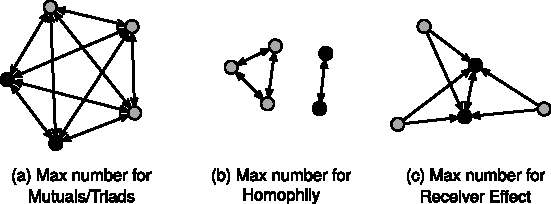
\includegraphics[width = .6\linewidth]{max-out-stats.pdf}
	%\caption[Examples of Networks with Saturated Statistics]{Networks with saturated statistics. All three networks have five vertices composed of two females (black vertices) and three males (gray vertices). Network (a) shows the required set of ties to saturate the \textit{Mutuals} and \textit{Transitive Triads} sufficient statistics, which actually coincides with a fully connected graph, containing $(5\times 4)/2 = 10$ mutual ties and $5 \times 4 \times 3 = 60$ transitive triads. Graph (b) shows the required configuration to saturate the \textit{Gender-Homophily} sufficient statistic, containing $3\times 2 + 2\times 1 = 8$ homophilic ties. Graph (c) shows the minimum arrangement to saturate the \textit{Gender-Receiver Effect} statistic, also having $4 + 4 = 8$ ties (so each female receives 4 ties).}
	\label{fig:maxout-gof-chapter}
\end{figure}
}

% % ------------------------------------------------------------------------------
\begin{frame}[t]
\frametitle{Concluding Remarks}

% \large {\bf Accomplished so far}
\begin{itemize}[<+->]
\item Paper 1: Phylogenetic models of gene functional evolution
  \begin{itemize}
  \item Parsimonious and biologically meaningful.
  \item Computationally scalable.
  \item Performance comparable to state-of-the-art alternatives.
  \item \textbf{Next steps:} Use ERGMs framework to break assumptions.
  \end{itemize}
\item Paper 2: ERGMs for small networks
  \begin{itemize}
  \item An extension to a well studied models for social networks.
  \item Small size allows exact calculations.
  \item Opens the door to a large set of methodological innovations.
  \item \textbf{Next steps:} GOF or extensions to large networks?
  \end{itemize}
\end{itemize}

\vfill
\footnotesize 
\uncover<11->{{\bf Accomplishments during the development of this work}
\begin{beamercolorbox}{conclusions}
\begin{itemize}
\item 6 journal publications (Journal of Open Source Software, Stata Journal, Journal of health and social behavior, Translational behavioral medicine, Social Science \& Medicine)
\item 11 packages/libraries built (ergmito, similR, gnet, fmcmc, slurmR, aphylo, polygons, pruner, netplot, rphyloxml, jsPhyloSVG)
\end{itemize}
\end{beamercolorbox}
}
\end{frame}

% % ------------------------------------------------------------------------------
\begin{frame}
\maketitle
\begin{center}
\scalebox{2}{\textcolor{uscgold}{Thanks!}}
\end{center}
\end{frame}

\renewcommand{\section}[2]{}%
\appendix
\begin{frame}[allowframebreaks]
\frametitle{References}
% \bibliographystyle{apacite}
% \bibliography{bibliography.bib}
\printbibliography
\end{frame}


% ------------------------------------------------------------------------------
% ------------------------------------------------------------------------------
% ------------------------------------------------------------------------------
% ------------------------------------------------------------------------------
% ------------------------------------------------------------------------------

% ------------------------------------------------------------------------------
\begin{frame}[label=aphylo-goexample]
\frametitle{The Gene Ontology Project}

Example of GO term

\begin{table}
\footnotesize
\begin{tabular}{lm{.6\linewidth}}
\toprule
\textbf{Accession} & GO:0060047 \\
\textbf{Name} & heart contraction \\
\textbf{Ontology} & biological\_process \\
\textbf{Synonyms} & heart beating, cardiac contraction, hemolymph circulation \\
\textbf{Alternate} & IDs None \\
\textbf{Definition} & The multicellular organismal process in which the heart decreases in volume in a 
characteristic way to propel blood through the body. Source: GOC:dph \\
\bottomrule
\end{tabular}
\caption{Heart Contraction Function. source: \href{http://amigo.geneontology.org/amigo/term/GO:0060047}{amigo.geneontology.org}}
\end{table}%\pause

You know what is interesting about this function?

\vfill \hfill \hyperlink{geneontology}{\beamerreturnbutton{go back}}

\end{frame}

% ------------------------------------------------------------------------------
\begin{frame}[t]

These four species have a gene with that function... \uncover<2->{and two of %
these are part of the same evolutionary tree!}

\vfill

\def\tmpwidth{.30\linewidth}
\begin{table}
\footnotesize
\begin{tabular}{*{2}{m{\tmpwidth}<\centering}}
\only<1>{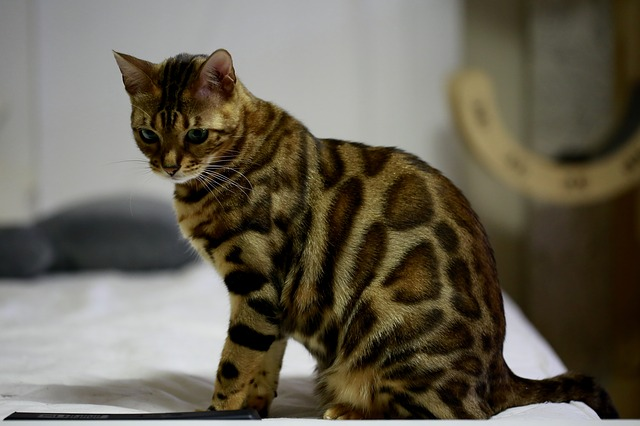
\includegraphics[width=.95\linewidth]{cat.jpg}} %
  \only<2->{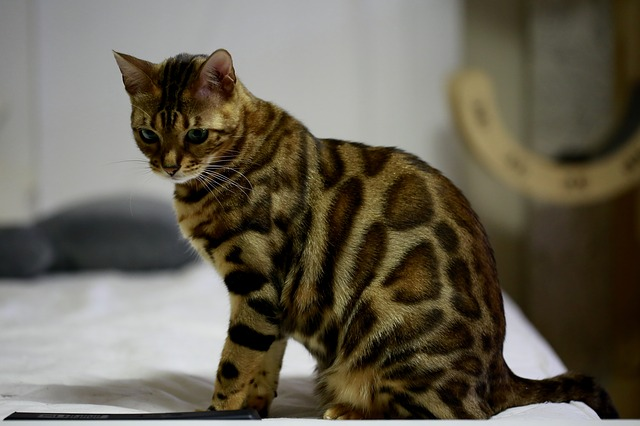
\includegraphics[width=.4\linewidth]{cat.jpg}} \linebreak Felis catus pthr10037 & %
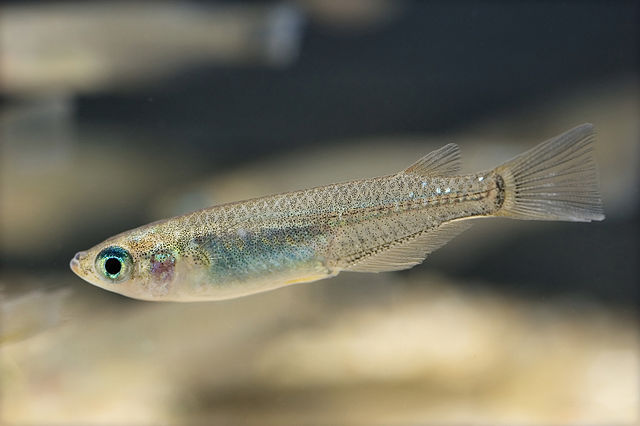
\includegraphics[width=1\linewidth]{Oryzias_latipes.jpg} \linebreak Oryzias latipes \textbf{pthr11521} \\ %
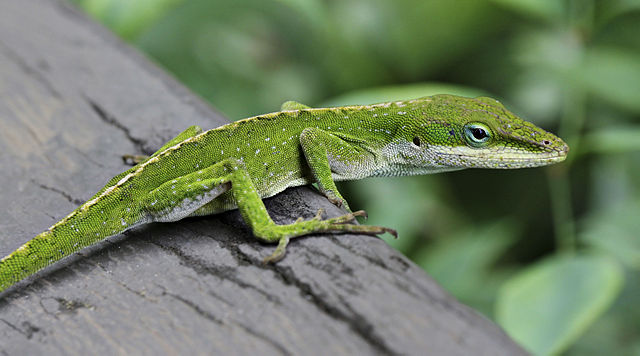
\includegraphics[width=1\linewidth]{Anole_Lizard.jpg} \linebreak Anolis carolinensis \textbf{pthr11521} & %
\only<1>{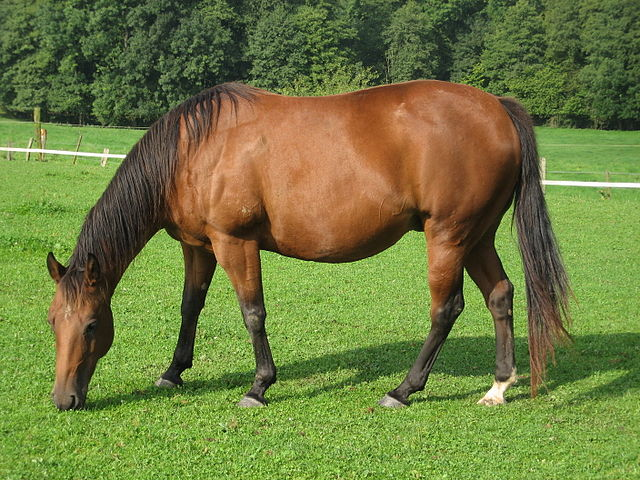
\includegraphics[width=.725\linewidth]{horse.jpg}} %
  \only<2->{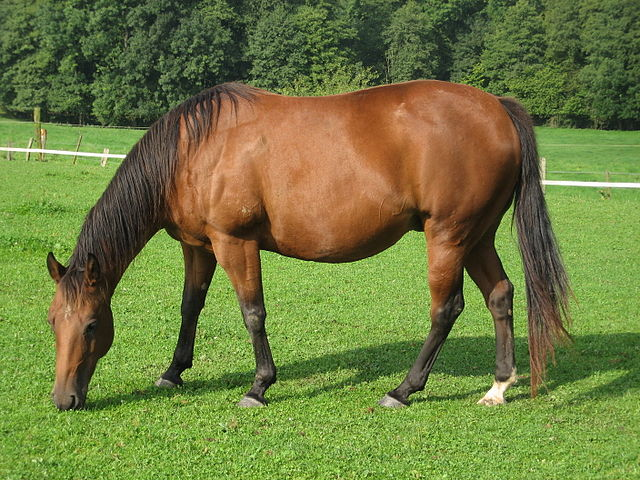
\includegraphics[width=.4\linewidth]{horse.jpg}} \linebreak Equus caballus pthr24356
\end{tabular}
\end{table}

\vfill \hfill \hyperlink{geneontology}{\beamerreturnbutton{go back}}

\end{frame}


% ------------------------------------------------------------------------------
\begin{frame}[label=other-models]
\frametitle{Predicting gene functions}
There various approaches for this, some to highlight
\begin{itemize}%[<+->]
\item Text analysis like in \cite{Pesaranghader2016}
\item Protein-protein interaction networks like in \cite{Oliver2000,Piovesan2015}.
\item Phylogenetic based like SIFTER \cite{Engelhardt2005,Engelhardt2011}.
\begin{itemize}
\item Parameters to estimate: $2^{2P}$, where $P$ is the number of functions.
\end{itemize}
\end{itemize}

\vfill \hfill (a nice literature review in \cite{Jiang2016,Yu2018})
\hyperlink{aphylographicalview}{\beamerreturnbutton{go back}}

\end{frame}


% ------------------------------------------------------------------------------
\begin{frame}[label=aphyloalgorithmicview]
\frametitle{An evolutionary model of gene functions (algorithmic view)}

\scalebox{.7}{

\begin{algorithm}[H]
\SetAlgoLined
\KwData{A phylogenetic tree, $\{\pi, \mu, \psi\}$(Model probabilities)}
\KwResult{An annotated tree}
%\pause
\For{$n \in PostOrder(N)$}{
  $\mbox{\bf\color{usccardinal}Nodes gain/loss function depending on their parent}$\;%\pause
  \Switch{class of $n$}{
    \uCase{root node}{
      Gain function with probability $\pi$\;
    }%\pause
    \uCase{interior node} {%\pause
      \lIf{Parent has the function}{Keep it with prob. $(1-\mu_1)$}%\pause
      \lElse{Gain it with prob. $\mu_0$}%\pause
    }
  }%\pause
  $\mbox{\bf\color{usccardinal}Finally, we allow for mislabeling}$\;%\pause
  \uIf{$n$ is leaf}{%\pause
    \lIf{has the function}{Mislabel with prob. $\psi_1$}%\pause
    \lElse{Mislabel with prob. $\psi_0$}%\pause
  }
}
\end{algorithm}
}

\vfill\hfill \hyperlink{aphylographicalview}{\beamergotobutton{go back}}


\end{frame}

% --------------------------
\begin{frame}[label=aphylo-pooled]

% latex table generated in R 3.6.3 by xtable 1.8-4 package
% Tue Apr 28 11:51:17 2020
\begin{table}[tb]
	\centering
	\begin{tabular}{m{.14\linewidth}*{3}{m{.14\linewidth}<\centering}}
		\toprule & \multicolumn{1}{c}{\textit{Pooled-data}} & \multicolumn{2}{c}{One-at-a-time} \\ \cmidrule(r){2-2}\cmidrule(r){3-4}
		& Beta prior & Unif. prior & Beta Prior \\ 
		\midrule
		\textit{Pooled-data} \\
		\hspace{2mm}Unif. prior & \cellcolor{blue!25}[-0.02,-0.01] & \cellcolor{blue!25}[-0.14,-0.10] & \cellcolor{blue!25}[-0.06,-0.03] \\ 
		\hspace{2mm}Beta prior &  - & \cellcolor{blue!25}[-0.12,-0.09] & \cellcolor{blue!25}[-0.04,-0.01] \\ 
		\textit{One-at-a-time} \\
		\hspace{2mm}Unif. prior &  - & - & \cellcolor{red!25}[\hphantom{-}0.06,\hphantom{-}0.09] \\ 
		\bottomrule
	\end{tabular}
	\caption[Differences in Mean Absolute Error]{Differences in Mean Absolute Error [MAE]. Each cell shows the 95\% confidence interval for the difference in MAE resulting from two methods (row method minus column method). Cells are color coded blue when the method on that row has a significantly small MAE than the method on that column; Conversely, cells are colored red when the method in that column outperforms the method in that row.  Overall, predictions calculated using the parameter estimates from \textit{pooled-data} predictions outperform \textit{one-at-a-time}.}
	\label{tab:vs-accuracy}
\end{table}

\end{frame}

% ------------------------------------------------------------------------------
\begin{frame}[label = duplicationvsspeciation]
\frametitle{Speciation}
\begin{figure}
\centering
\def\svgwidth{.8\linewidth}
\tiny
% Source 
\input{fig/Drosophila_speciation_experiment.pdf_tex}
\caption{\cite{Dodd1989}: After one year of isolation, flies showed a significant level or assortativity in mating (\href{https://commons.wikimedia.org/wiki/File:Drosophila_speciation_experiment.svg}{wikimedia})}
\end{figure}

\vfill\hfill \hyperlink{aphylographicalview}{\beamerreturnbutton{go back}}

\end{frame}

\begin{frame}
\frametitle{Duplication}
\begin{figure}
\centering
\def\svgwidth{.6\linewidth}
\tiny
% Source : https://en.wikipedia.org/wiki/File:Evolution_fate_duplicate_genes_-_vector.svg
\input{fig/Evolution_fate_duplicate_genes_-_vector.pdf_tex}
\caption{A key part of molecular innovation, gene duplication provides opportunity for new functions to emerge (\href{https://en.wikipedia.org/wiki/File:Evolution_fate_duplicate_genes_-_vector.svg}{wikimedia})}
\end{figure}

\vfill\hfill \hyperlink{aphylographicalview}{\beamerreturnbutton{go back}}

\end{frame}





% ------------------------------------------------------------------------------
\begin{frame}[label=mcmle]
\frametitle{ERGMs: The MC-MLE approach}

One of the most popular methods for estimating ERGMs is the MC-MLE approach (citations here)

This consists on the following steps

\begin{enumerate}
\item Start from a sensible guess on what should be the population parameters
(usually done using pseudo-MLE estimation)
\item While the algorithm doesn't converge, do:
  \begin{enumerate}
  \item Simulate a stream of networks with the current state of the parameter,
  $\theta_t$
  \item Using the law of large numbers, approximate the ratio of likelihoods 
  based on the parameter $\theta_t$, this is the objective function
  \item Update the parameter by a Newton-Raphson step
  \item Next iteration
  \end{enumerate}
\end{enumerate}

\vfill\hfill \hyperlink{art}{\beamerreturnbutton{go back}}


\end{frame}



% ------------------------------------------------------------------------------
\begin{frame}[label=ergmitodgp]
\frametitle{Paper 2 Simulation Studies}

We performed a simulation study with the following features:

\begin{itemize}%[<+->]
\item Draw 20,000 samples of groups of small networks
\item Each group had prescribed: (model parameters, number of networks, sizes of the networks)
\item Each group could have from 5 to 300 small networks
\item We estimated the models using MC-MLE and MLE.
\end{itemize}

\vfill\hfill\hyperlink{ergmitoexample}{\beamerreturnbutton{go back}}

\end{frame}



% ------------------------------------------------------------------------------
\begin{frame}[label=ergmito-bias]
\frametitle{Paper 2 Simulation Studies: Empirical Bias}

\begin{figure}
\centering
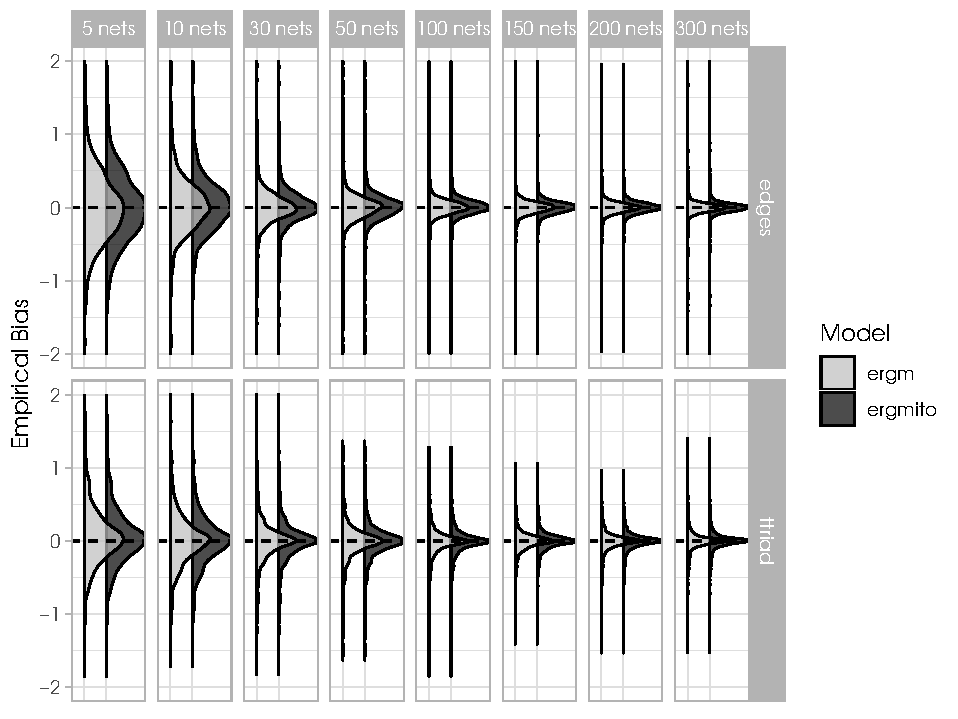
\includegraphics[width=.6\linewidth]{bias-02-various-sizes-4-5-ttriad.pdf}
\end{figure}

%\vfill\hfill \hyperlink{ergmitoexperiment}{\beamerreturnbutton{go back}}

\end{frame}

\end{document}

